% This LaTeX was auto-generated from MATLAB code.
% To make changes, update the MATLAB code and export to LaTeX again.

\documentclass{article}

\usepackage[utf8]{inputenc}
\usepackage[T1]{fontenc}
\usepackage{lmodern}
\usepackage{graphicx}
\usepackage{color}
\usepackage{listings}
\usepackage{hyperref}
\usepackage{amsmath}
\usepackage{amsfonts}
\usepackage{epstopdf}
\usepackage{matlab}

\sloppy
\epstopdfsetup{outdir=./}
\graphicspath{ {./FilterIntroductionExample_images/} }

\begin{document}

\matlabtitle{Practical Introduction to Digital Filtering}

\begin{par}
\begin{flushleft}
This example shows how to design, analyze, and apply a digital filter to your data. It will help you answer questions such as: how do I compensate for the delay introduced by a filter?, How do I avoid distorting my signal?, How do I remove unwanted content from my signal?, How do I differentiate my signal?, and How do I integrate my signal?
\end{flushleft}
\end{par}

\begin{par}
\begin{flushleft}
Filters can be used to shape the signal spectrum in a desired way or to perform mathematical operations such as differentiation and integration. In what follows you will learn some practical concepts that will ease the use of filters when you need them.
\end{flushleft}
\end{par}

\begin{par}
\begin{flushleft}
This example focuses on applications of digital filters rather than on their design. If you want to learn more about how to design digital filters see the \href{../../../signal/sigdemos/html/FilterDesignIntroductionExample.html}{"Practical Introduction to Digital Filter Design"} example.
\end{flushleft}
\end{par}

\matlabheading{Compensating for Delay Introduced by Filtering}

\begin{par}
\begin{flushleft}
Digital filters introduce delay in your signal. Depending on the filter characteristics, the delay can be constant over all frequencies, or it can vary with frequency. The type of delay determines the actions you have to take to compensate for it. The \textbf{grpdelay} function allows you to look at the filter delay as a function of frequency. Looking at the output of this function allows you to identify if the delay of the filter is constant or if it varies with frequency (i.e. if it is frequency-dependent).
\end{flushleft}
\end{par}

\begin{par}
\begin{flushleft}
Filter delay that is constant over all frequencies can be easily compensated for by shifting the signal in time. FIR filters usually have constant delay. On the other hand, delay that varies with frequency causes phase distortion and can alter a signal waveform significantly. Compensating for frequency-dependent delay is not as trivial as for the constant delay case. IIR filters introduce frequency-dependent delay.
\end{flushleft}
\end{par}

\begin{par}
\begin{flushleft}
\textbf{Compensating for Constant Filter Delay}
\end{flushleft}
\end{par}

\begin{par}
\begin{flushleft}
As mentioned before, you can measure the group of delay of the filter to verify that it is a constant function of frequency. You can use the \textbf{grpdelay} function to measure the filter delay, D, and compensate for this delay by appending D zeros to the input signal and shifting the output signal in time by D samples.
\end{flushleft}
\end{par}

\begin{par}
\begin{flushleft}
Consider a noisy electrocardiogram signal that you want to filter to remove high frequency noise above 75 Hz. You want to apply an FIR lowpass filter and compensate for the filter delay so that the noisy and filtered signals are aligned correctly and can be plotted on top of each other for comparison.
\end{flushleft}
\end{par}

\begin{matlabcode}
Fs = 500;                    % sample rate in Hz
N = 500;                     % number of signal samples
rng default;
x = ecg(N)'+0.25*randn(N,1); % noisy waveform
t = (0:N-1)/Fs;              % time vector

% Design a 70th order lowpass FIR filter with cutoff frequency of 75 Hz.

Fnorm = 75/(Fs/2);           % Normalized frequency
df = designfilt('lowpassfir','FilterOrder',70,'CutoffFrequency',Fnorm);
\end{matlabcode}


\begin{par}
\begin{flushleft}
Plot the group delay of the filter to verify that it is constant across all frequencies indicating that the filter is linear phase. Use the group delay to measure the delay of the filter.
\end{flushleft}
\end{par}

\begin{matlabcode}
grpdelay(df,2048,Fs)   % plot group delay
\end{matlabcode}
\begin{center}
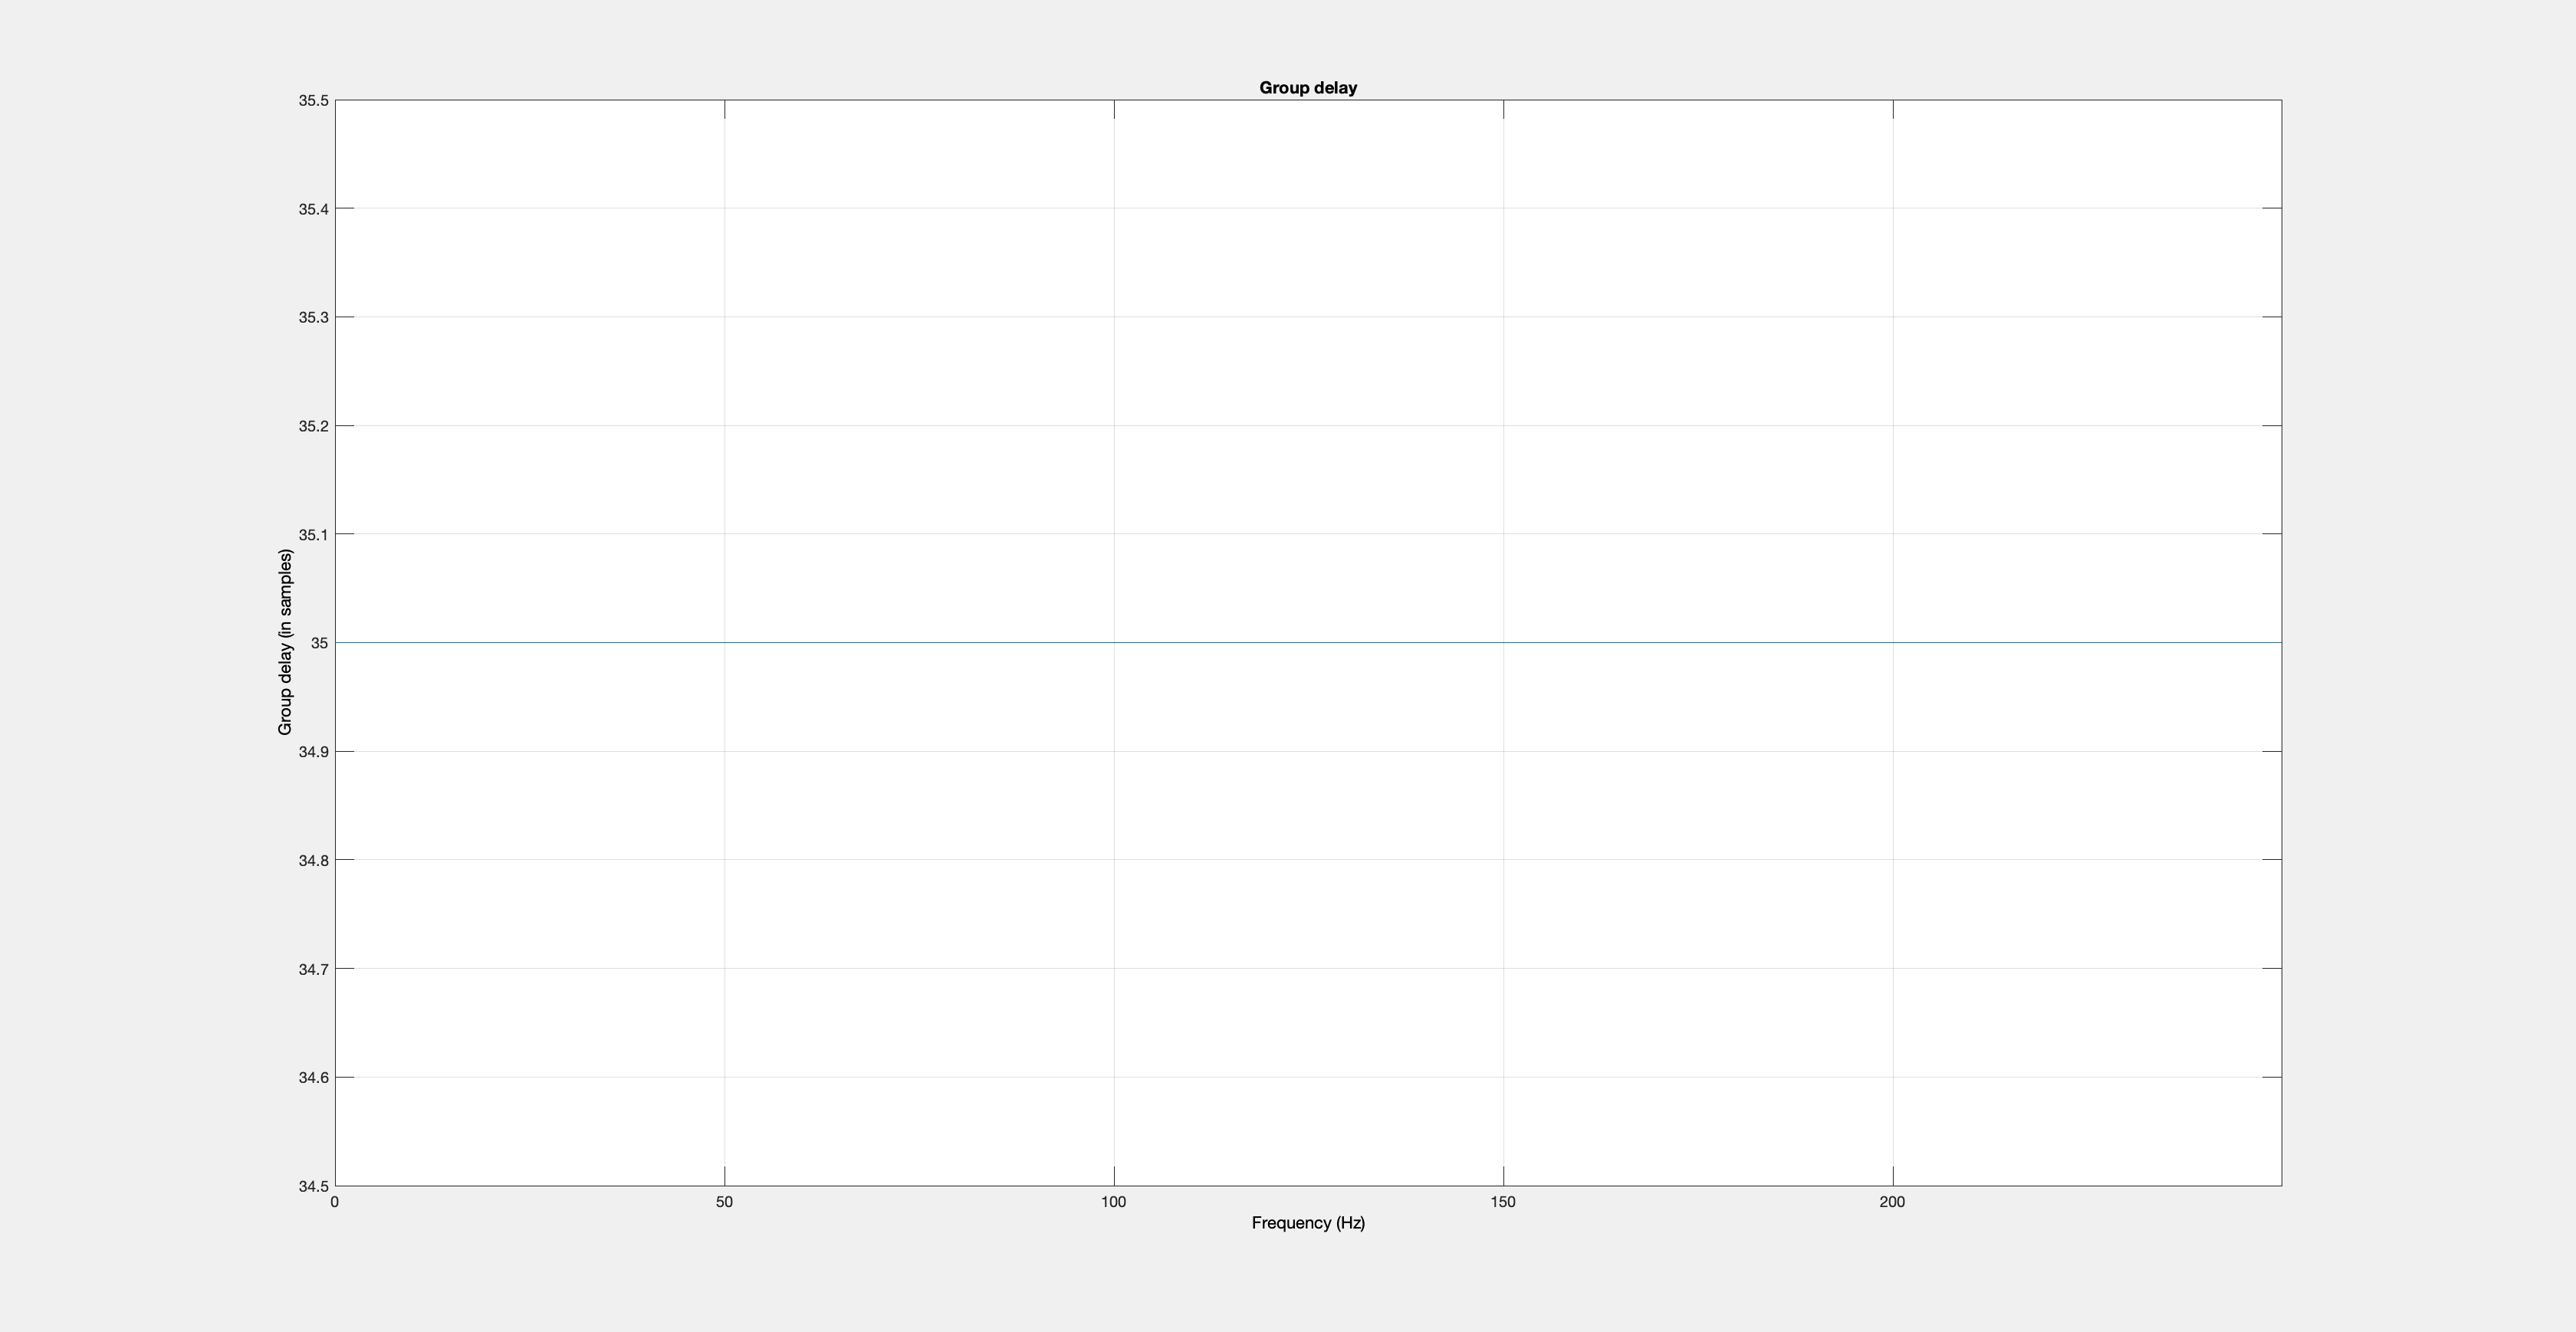
\includegraphics[width=\maxwidth{123.13095835423984em}]{figure_0}
\end{center}
\begin{matlabcode}
D = mean(grpdelay(df)) % filter delay in samples
\end{matlabcode}
\begin{matlaboutput}
D = 35
\end{matlaboutput}


\begin{par}
\begin{flushleft}
Before filtering, append D zeros at the end of the input data vector, x. This ensures that all the useful samples are flushed out of the filter, and that the input signal and the delay-compensated output signal have the same length. Filter the data and compensate for the delay by shifting the output signal by D samples. This last step effectively removes the filter transient.
\end{flushleft}
\end{par}

\begin{matlabcode}
y = filter(df,[x; zeros(D,1)]); % Append D zeros to the input data
y = y(D+1:end);                  % Shift data to compensate for delay

figure
plot(t,x,t,y,'r','linewidth',1.5);
title('Filtered Waveforms');
xlabel('Time (s)')
legend('Original Noisy Signal','Filtered Signal');
grid on
axis tight
\end{matlabcode}
\begin{center}
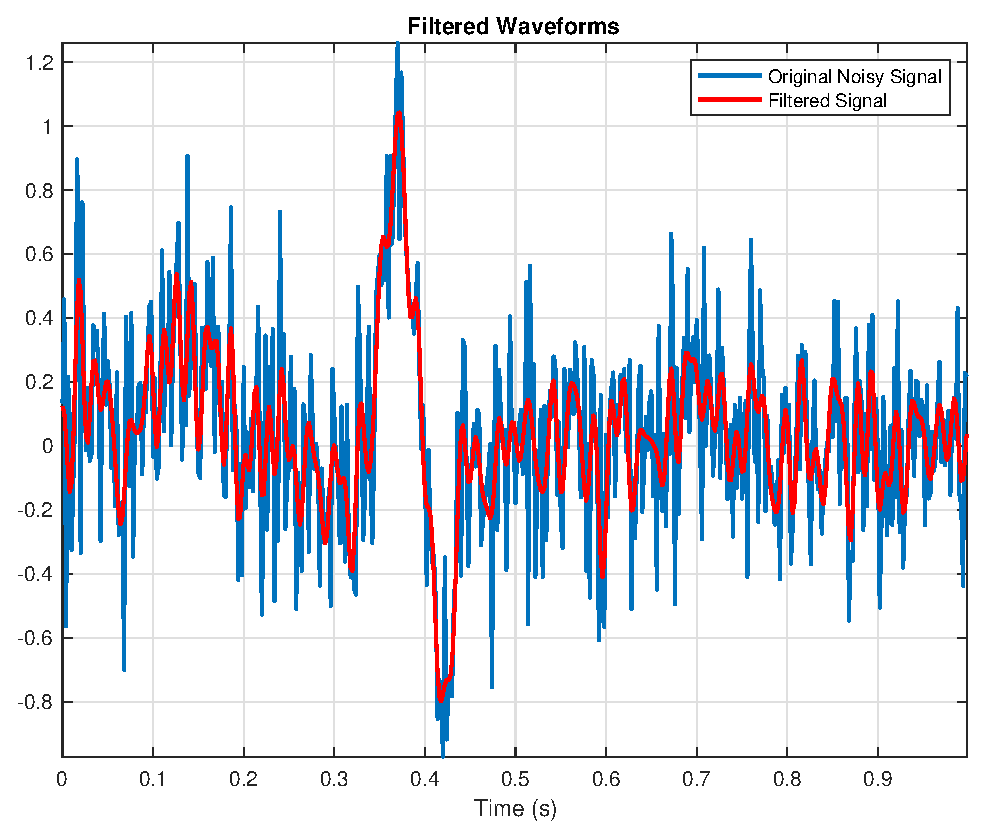
\includegraphics[width=\maxwidth{56.196688409433015em}]{figure_1}
\end{center}


\begin{par}
\begin{flushleft}
\textbf{Compensating for Frequency-Dependent Delay}
\end{flushleft}
\end{par}

\begin{par}
\begin{flushleft}
Frequency-dependent delay causes phase distortion in the signal. Compensating for this type of delay is not as trivial as for the constant delay case. If your application allows off-line processing, you can remove the frequency-dependent delay by implementing zero-phase filtering using the \textbf{filtfilt} function. \textbf{filtfilt} performs zero-phase filtering by processing the input data in both the forward and reverse directions. The main effect is that you obtain zero-phase distortion, i.e., you filter data with an equivalent filter that has a constant delay of 0 samples. Other effects are that you get a filter transfer function which equals the squared magnitude of the original filter transfer function, and a filter order that is double the order of the original filter.
\end{flushleft}
\end{par}

\begin{par}
\begin{flushleft}
Consider the ECG signal defined in the previous section. Filter this signal with and without delay compensation.
\end{flushleft}
\end{par}

\begin{matlabcode}
% Design a 7th order lowpass IIR elliptic filter with cutoff frequency
% of 75 Hz.

Fnorm = 75/(Fs/2); % Normalized frequency
df = designfilt('lowpassiir',...
               'PassbandFrequency',Fnorm,...
               'FilterOrder',7,...
               'PassbandRipple',1,...
               'StopbandAttenuation',60);
\end{matlabcode}


\begin{par}
\begin{flushleft}
Plot the group delay of the filter and notice that it varies with frequency indicating that the filter delay is frequency-dependent.
\end{flushleft}
\end{par}

\begin{matlabcode}
grpdelay(df,2048,'half',Fs)
\end{matlabcode}
\begin{center}
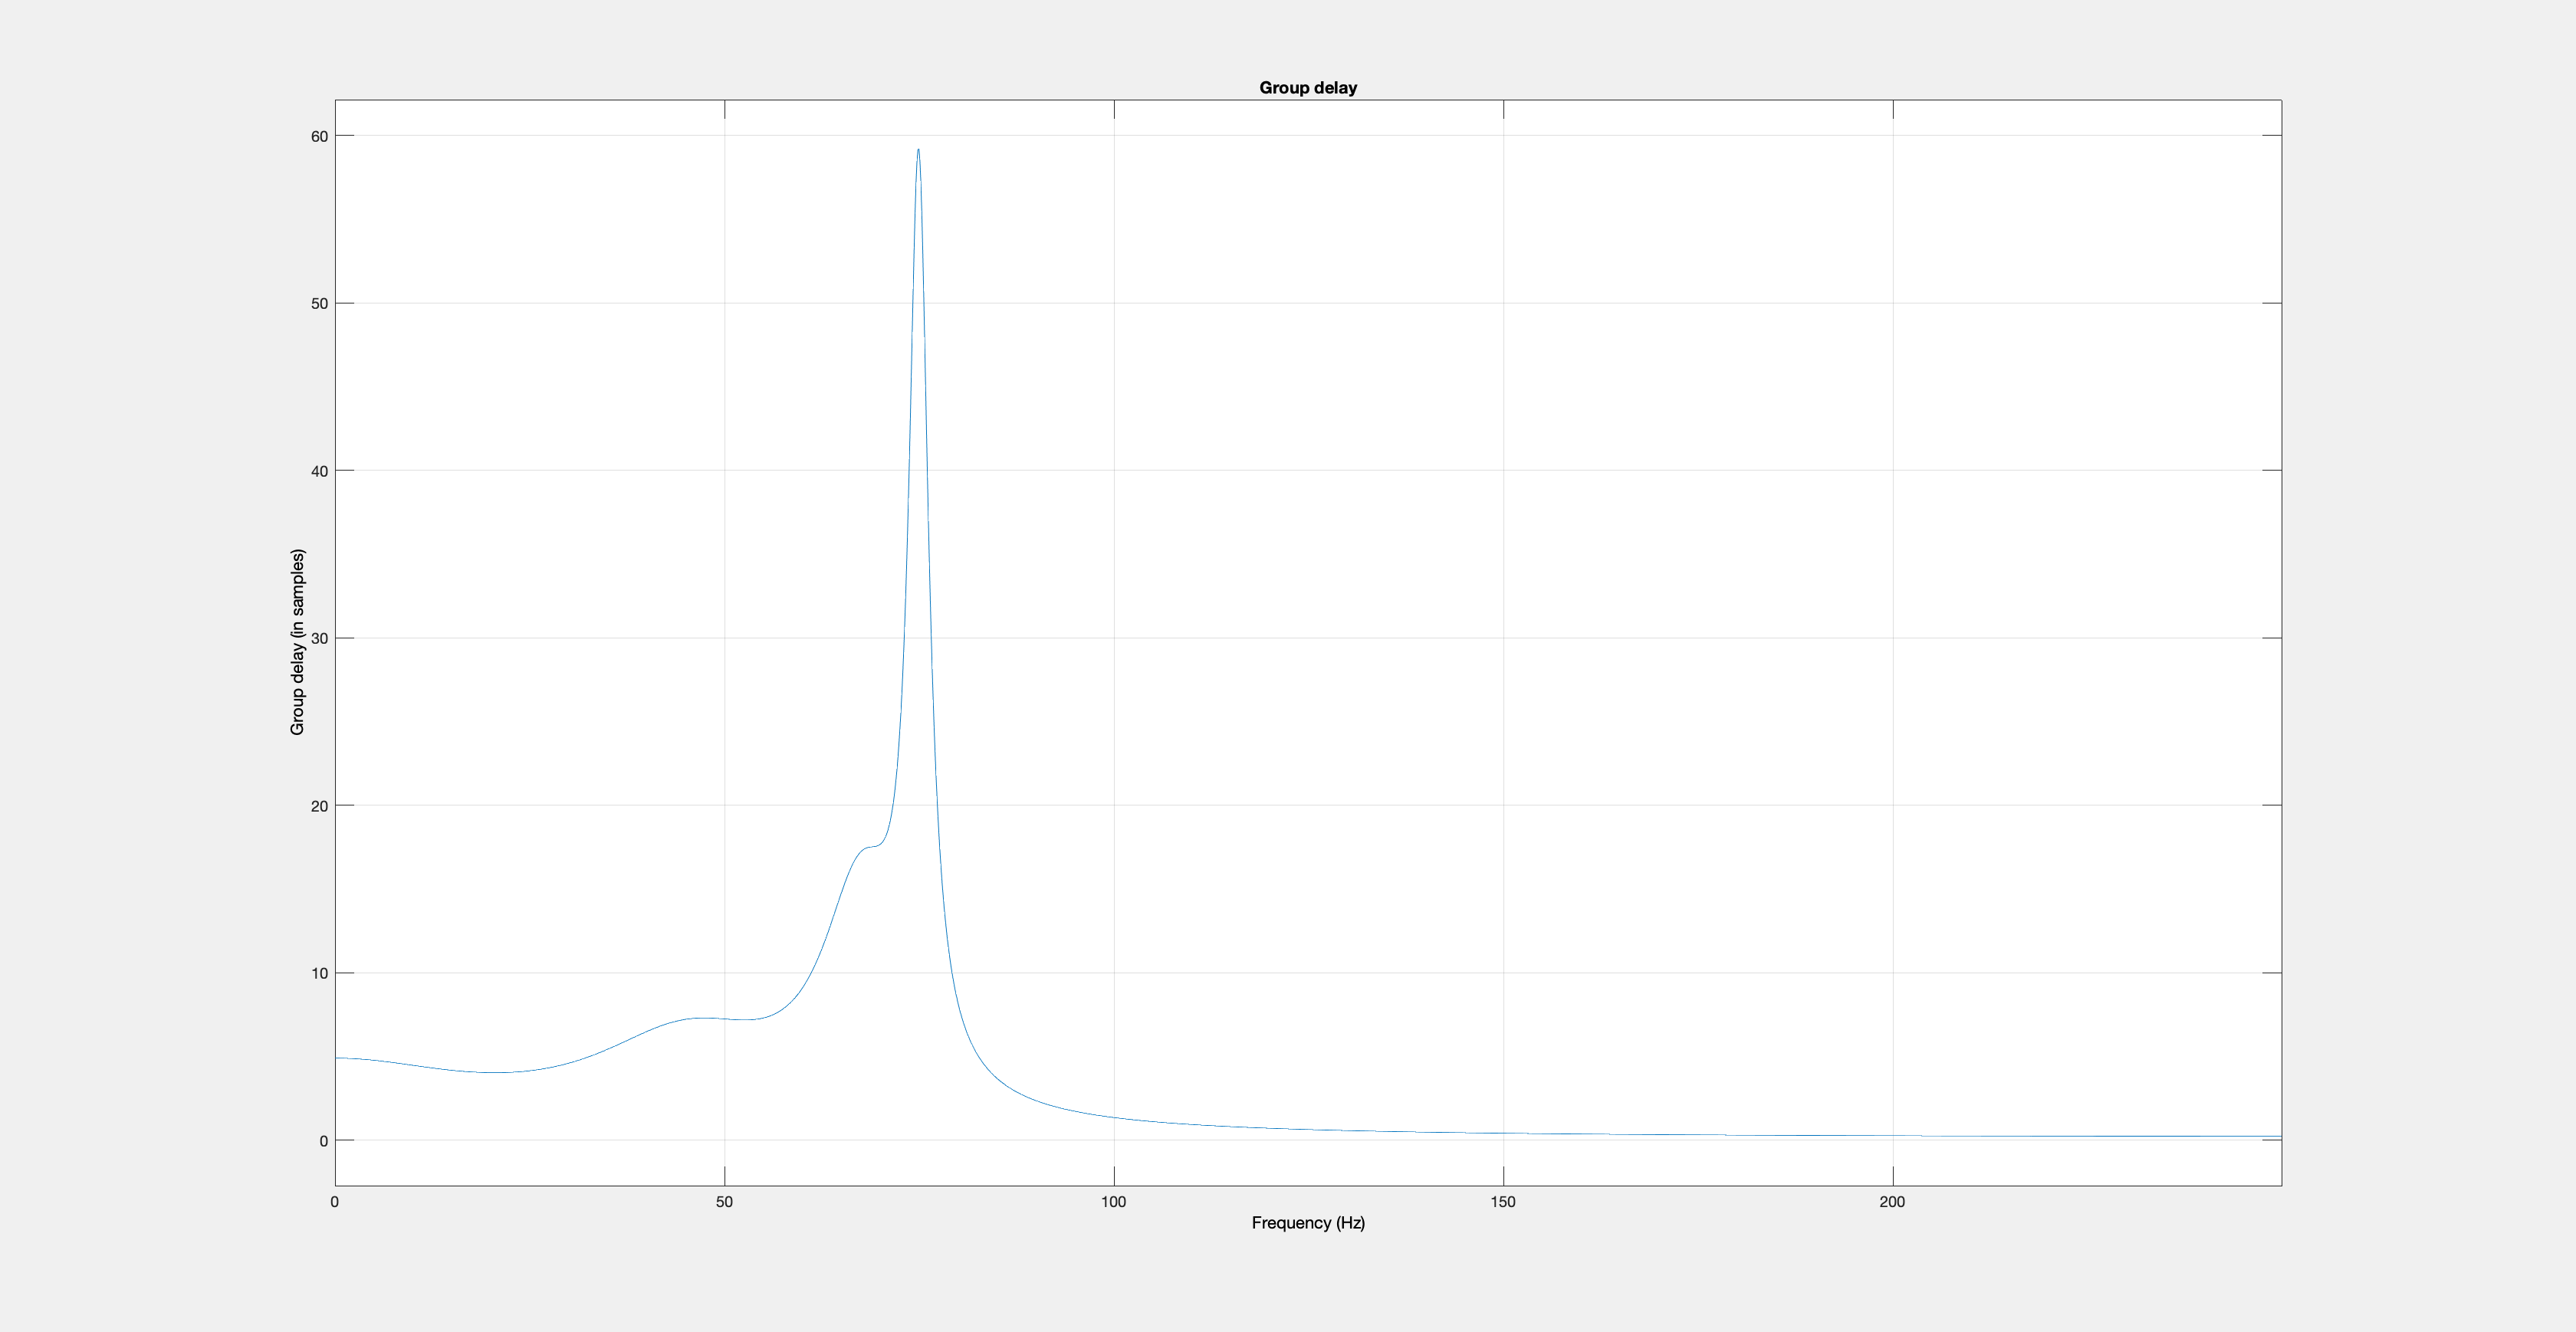
\includegraphics[width=\maxwidth{123.13095835423984em}]{figure_2}
\end{center}


\begin{par}
\begin{flushleft}
Filter the data and look at the effects of each filter implementation on the time signal.
\end{flushleft}
\end{par}

\begin{matlabcode}
y1 = filter(df,x);    % non-linear phase filter - no delay compensation
y2 = filtfilt(df,x);  % zero-phase implementation - delay compensation

figure
plot(t,x);
hold on
plot(t,y1,'r','linewidth',1.5);
plot(t,y2,'g','linewidth',1.5);
title('Filtered Waveforms');
xlabel('Time (s)')
legend('Original Signal','Non-linear phase IIR output',...
  'Zero-phase IIR output');
ax = axis;
axis([0.25 0.55 ax(3:4)])
grid on
\end{matlabcode}
\begin{center}
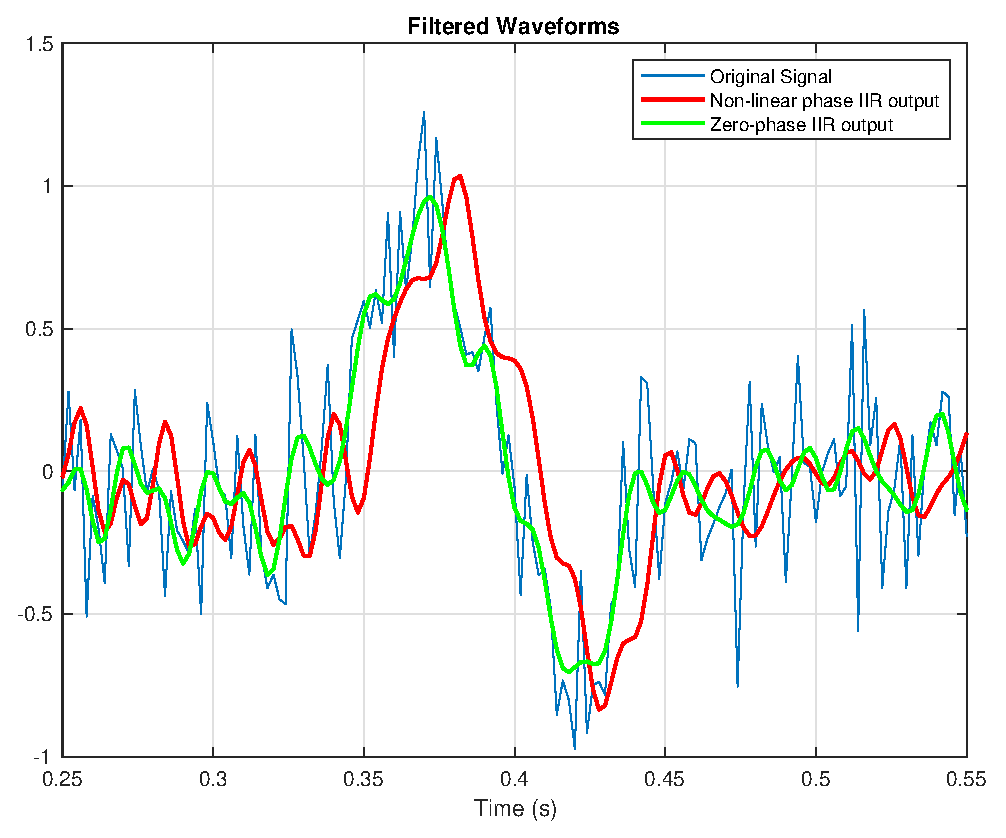
\includegraphics[width=\maxwidth{56.196688409433015em}]{figure_3}
\end{center}

\begin{par}
\begin{flushleft}
Notice how zero-phase filtering effectively removes the filter delay.
\end{flushleft}
\end{par}

\begin{par}
\begin{flushleft}
Zero-phase filtering is a great tool if your application allows for the non-causal forward/backward filtering operations, and for the change of the filter response to the square of the original response.
\end{flushleft}
\end{par}

\begin{par}
\begin{flushleft}
Filters that introduce constant delay are linear phase filters. Filters that introduce frequency-dependent delay are non-linear phase filters.
\end{flushleft}
\end{par}


\matlabheading{Removing Unwanted Spectral Content from a Signal}

\begin{par}
\begin{flushleft}
Filters are commonly used to remove unwanted spectral content from a signal. You can choose from a variety of filters to do this. You choose a lowpass filter when you want to remove high frequency content, or a highpass filter when you want to remove low frequency content. You can also choose a bandpass filter to remove low and high frequency content while leaving an intermediate band of frequencies intact. You choose a bandstop filter when you want to remove frequencies over a given band.
\end{flushleft}
\end{par}

\begin{par}
\begin{flushleft}
Consider an audio signal that has a power-line hum and white noise. The power-line hum is caused by a 60 Hz tone. White noise is a signal that exists across all the audio bandwidth. 
\end{flushleft}
\end{par}

\begin{par}
\begin{flushleft}
Load the audio signal.
\end{flushleft}
\end{par}

\begin{matlabcode}
Fs = 44100; % Sample rate
y = audioread('noisymusic.wav');
\end{matlabcode}


\begin{par}
\begin{flushleft}
Plot the power spectrum of the signal. The red triangular marker shows the strong 60 Hz tone interfering with the audio signal. 
\end{flushleft}
\end{par}

\begin{matlabcode}
[P,F] = pwelch(y,ones(8192,1),8192/2,8192,Fs,'power');
helperFilterIntroductionPlot1(F,P,[60 60],[-9.365 -9.365],...
  {'Original signal power spectrum', '60 Hz Tone'})
\end{matlabcode}
\begin{center}
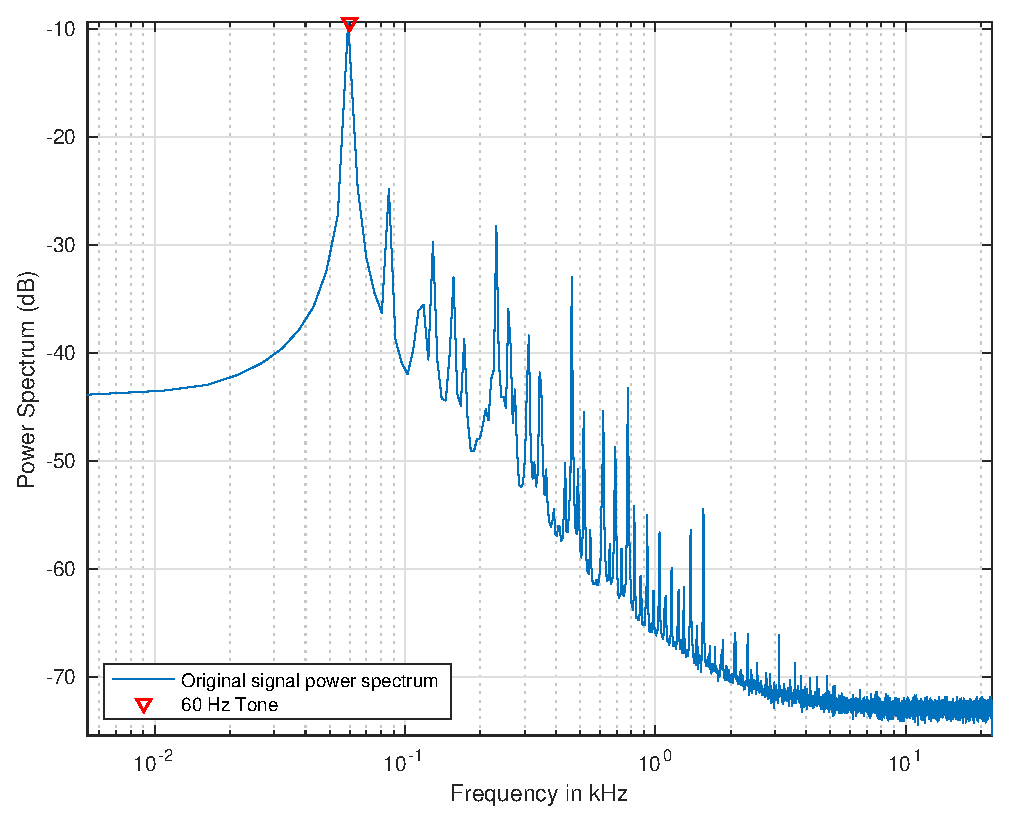
\includegraphics[width=\maxwidth{56.196688409433015em}]{figure_4}
\end{center}


\begin{par}
\begin{flushleft}
You can first remove as much white noise spectral content as possible using a lowpass filter. The passband of the filter should be set to a value that offers a good trade-off between noise reduction and audio degradation due to loss of high frequency content. Applying the lowpass filter before removing the 60 Hz hum is very convenient since you will be able to downsample the band-limited signal. The lower rate signal will allow you to design a sharper and narrower 60 Hz bandstop filter with a smaller filter order.
\end{flushleft}
\end{par}

\begin{par}
\begin{flushleft}
Design a lowpass filter with passband frequency of 1 kHz, and stopband frequency of 1.4 kHz. Choose a minimum order design.
\end{flushleft}
\end{par}

\begin{matlabcode}
Fp = 1e3;    % Passband frequency in Hz
Fst = 1.4e3; % Stopband frequency in Hz
Ap = 1;      % Passband ripple in dB
Ast = 95;    % Stopband attenuation in dB

% Design the filter 
df = designfilt('lowpassfir','PassbandFrequency',Fp,...
                'StopbandFrequency',Fst,'PassbandRipple',Ap,...
                'StopbandAttenuation',Ast,'SampleRate',Fs);

% Analyze the filter response
hfvt = fvtool(df,'Fs',Fs,'FrequencyScale','log',...
  'FrequencyRange','Specify freq. vector','FrequencyVector',F);
\end{matlabcode}
\begin{center}
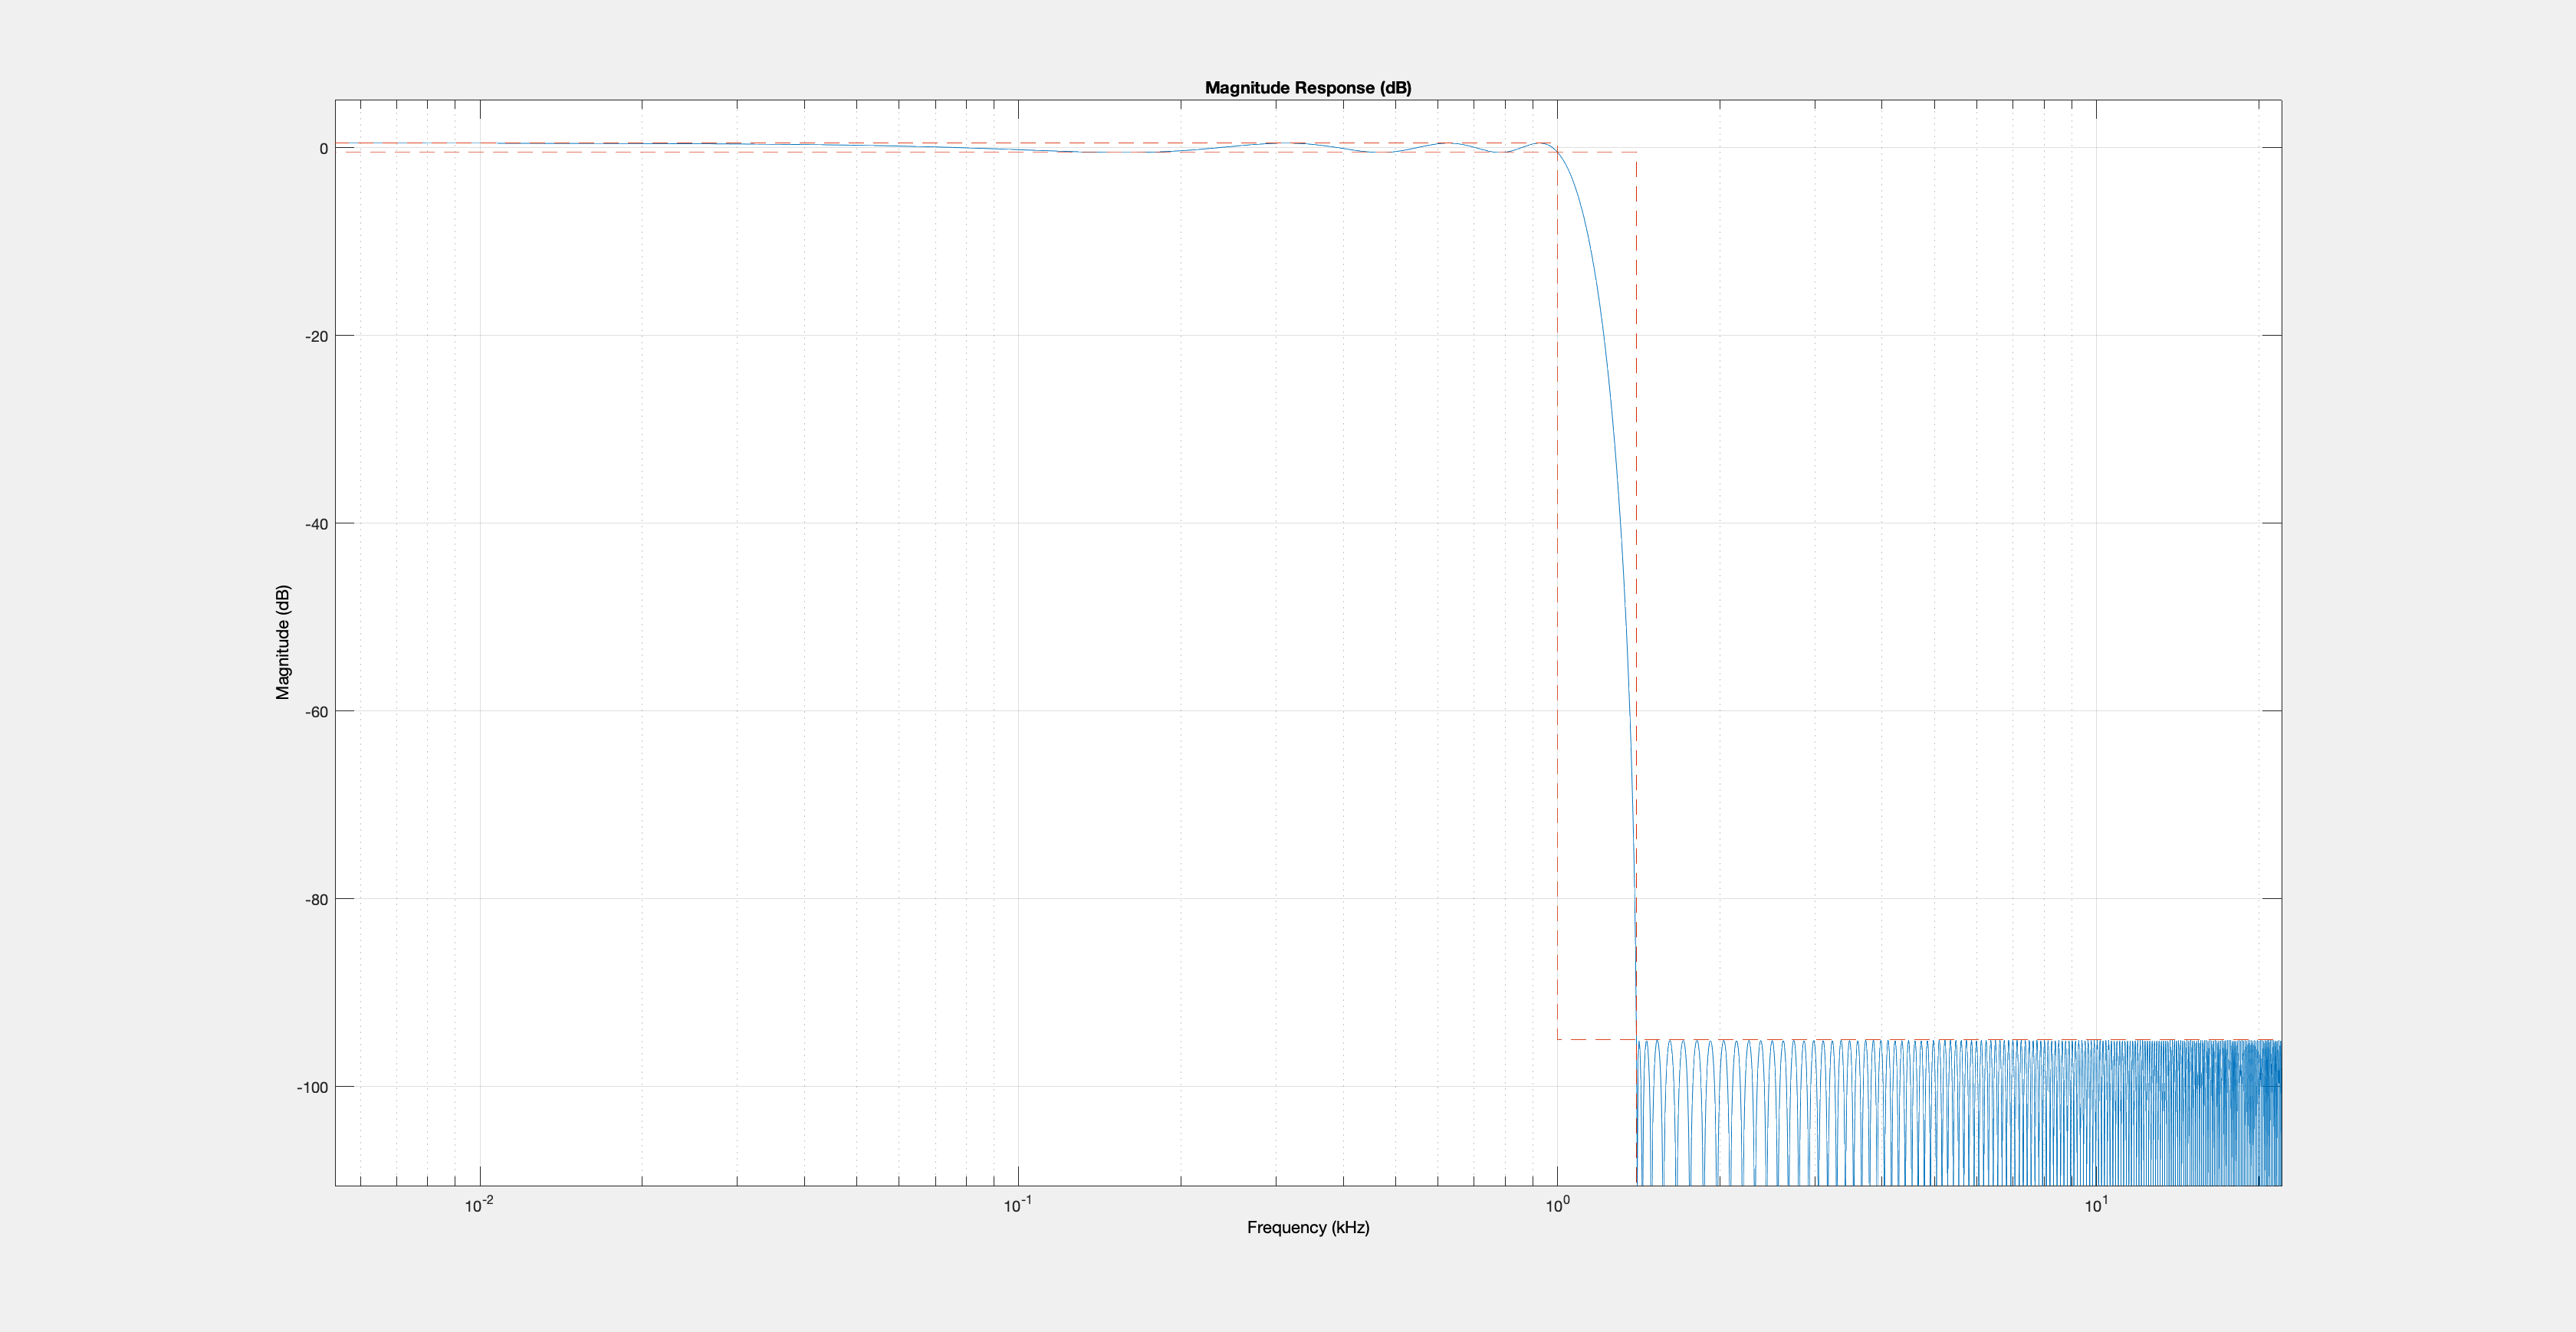
\includegraphics[width=\maxwidth{123.13095835423984em}]{figure_5}
\end{center}


\begin{matlabcode}
% Filter the data and compensate for delay
D = mean(grpdelay(df)); % filter delay
ylp = filter(df,[y; zeros(D,1)]);
ylp = ylp(D+1:end);

close(hfvt)
\end{matlabcode}


\begin{par}
\begin{flushleft}
Look at the spectrum of the lowpass filtered signal. Note how the frequency content above 1400 Hz has been removed. 
\end{flushleft}
\end{par}

\begin{matlabcode}
[Plp,Flp] = pwelch(ylp,ones(8192,1),8192/2,8192,Fs,'power');
helperFilterIntroductionPlot1(F,P,Flp,Plp,...
  {'Original signal','Lowpass filtered signal'})
\end{matlabcode}
\begin{center}
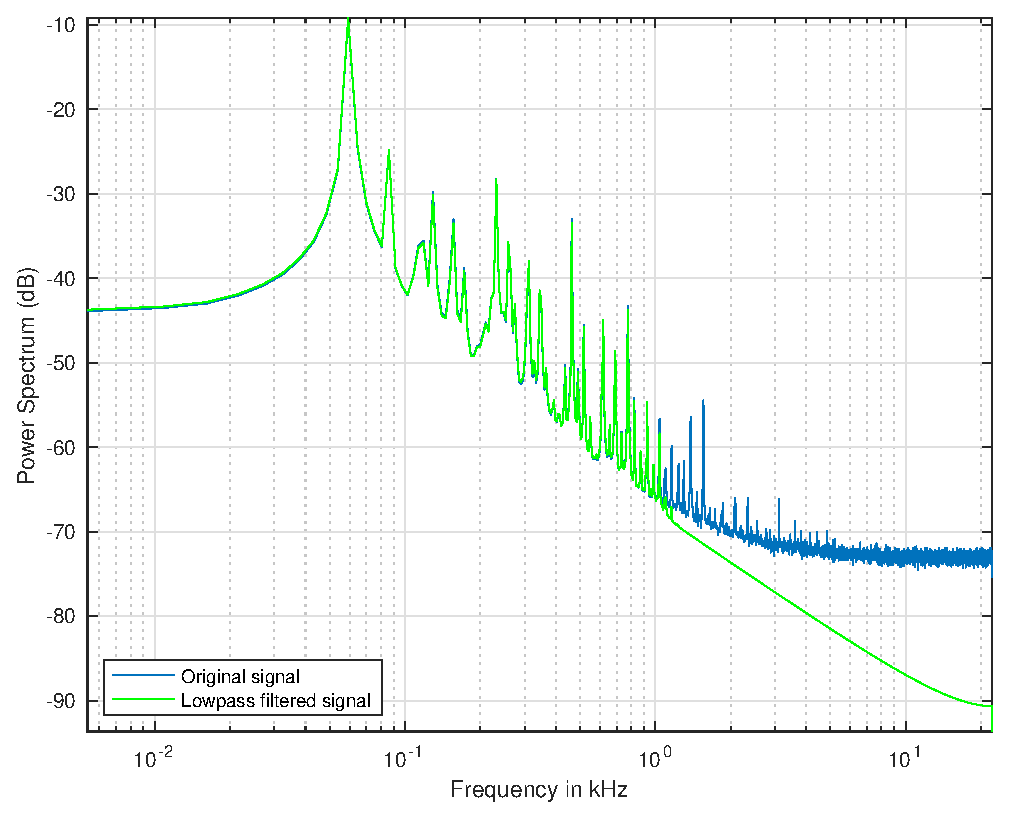
\includegraphics[width=\maxwidth{56.196688409433015em}]{figure_6}
\end{center}


\begin{par}
\begin{flushleft}
From the power spectrum plot above, you can see that the maximum non-negligible frequency content of the lowpass filtered signal is at 1400 Hz. By the sampling theorem, a sample frequency of 2*1400 = 2800 Hz would suffice to represent the signal correctly, you however, are using a sample rate of 44100 Hz which is a waste since you will need to process more samples than those necessary. You can downsample the signal to reduce the sample rate and reduce the computational load by reducing the number of samples that you need to process. A lower sample rate will also allow you to design a sharper and narrower bandstop filter, needed to remove the 60 Hz noise, with a smaller filter order.
\end{flushleft}
\end{par}

\begin{par}
\begin{flushleft}
Downsample the lowpass filtered signal by a factor of 10 to obtain a sample rate of Fs/10 = 4.41 kHz. Plot the spectrum of the signal before and after downsampling.
\end{flushleft}
\end{par}

\begin{matlabcode}
Fs = Fs/10;
yds = downsample(ylp,10);

[Pds,Fds] = pwelch(yds,ones(8192,1),8192/2,8192,Fs,'power');
helperFilterIntroductionPlot1(F,P,Fds,Pds,...
  {'Signal sampled at 44100 Hz', 'Downsampled signal, Fs = 4410 Hz'})
\end{matlabcode}
\begin{center}
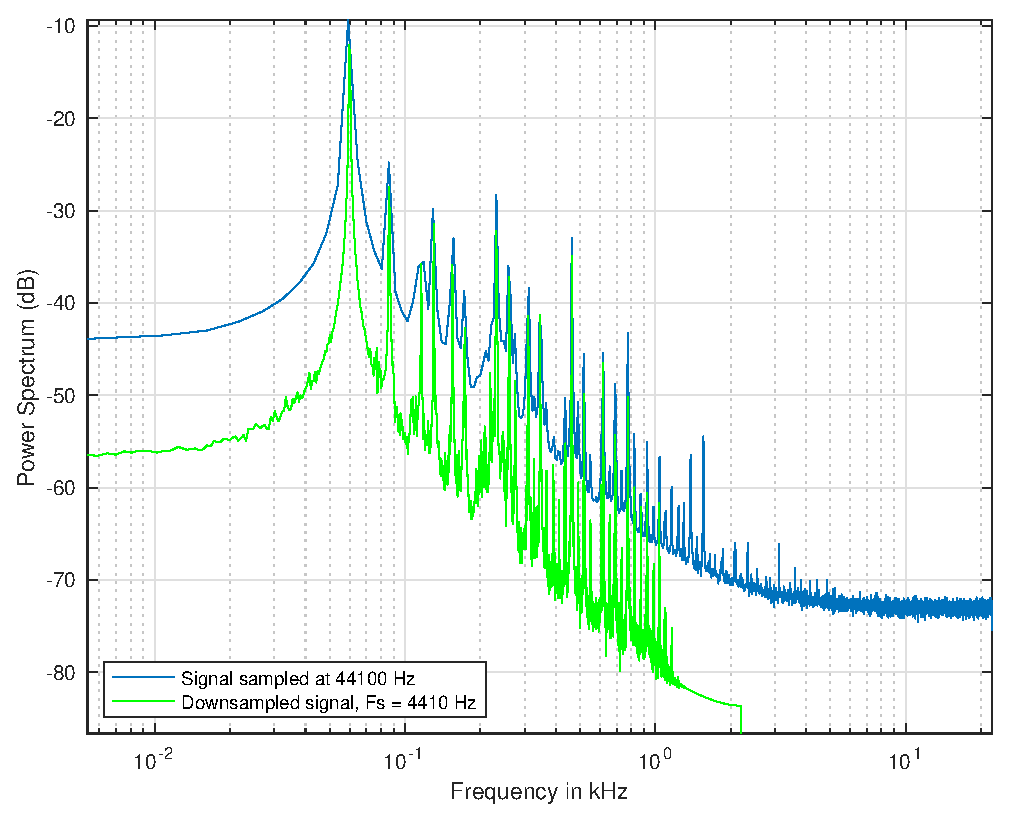
\includegraphics[width=\maxwidth{56.196688409433015em}]{figure_7}
\end{center}


\begin{par}
\begin{flushleft}
Now remove the 60 Hz tone using an IIR bandstop filter. Let the stopband have a width of 4 Hz centered at 60 Hz. We choose an IIR filter to achieve a sharp frequency notch, small passband ripple, and a relatively low order. Process the data using \textbf{filtfilt} to avoid phase distortion.
\end{flushleft}
\end{par}

\begin{matlabcode}
% Design the filter
df = designfilt('bandstopiir','PassbandFrequency1',55,...
               'StopbandFrequency1',58,'StopbandFrequency2',62,...
               'PassbandFrequency2',65,'PassbandRipple1',1,...
               'StopbandAttenuation',60,'PassbandRipple2',1,...
               'SampleRate',Fs,'DesignMethod','ellip');                          

% Analyze the magnitude response
hfvt = fvtool(df,'Fs',Fs,'FrequencyScale','log',...
  'FrequencyRange','Specify freq. vector','FrequencyVector',Fds(Fds>F(2)));
\end{matlabcode}
\begin{center}
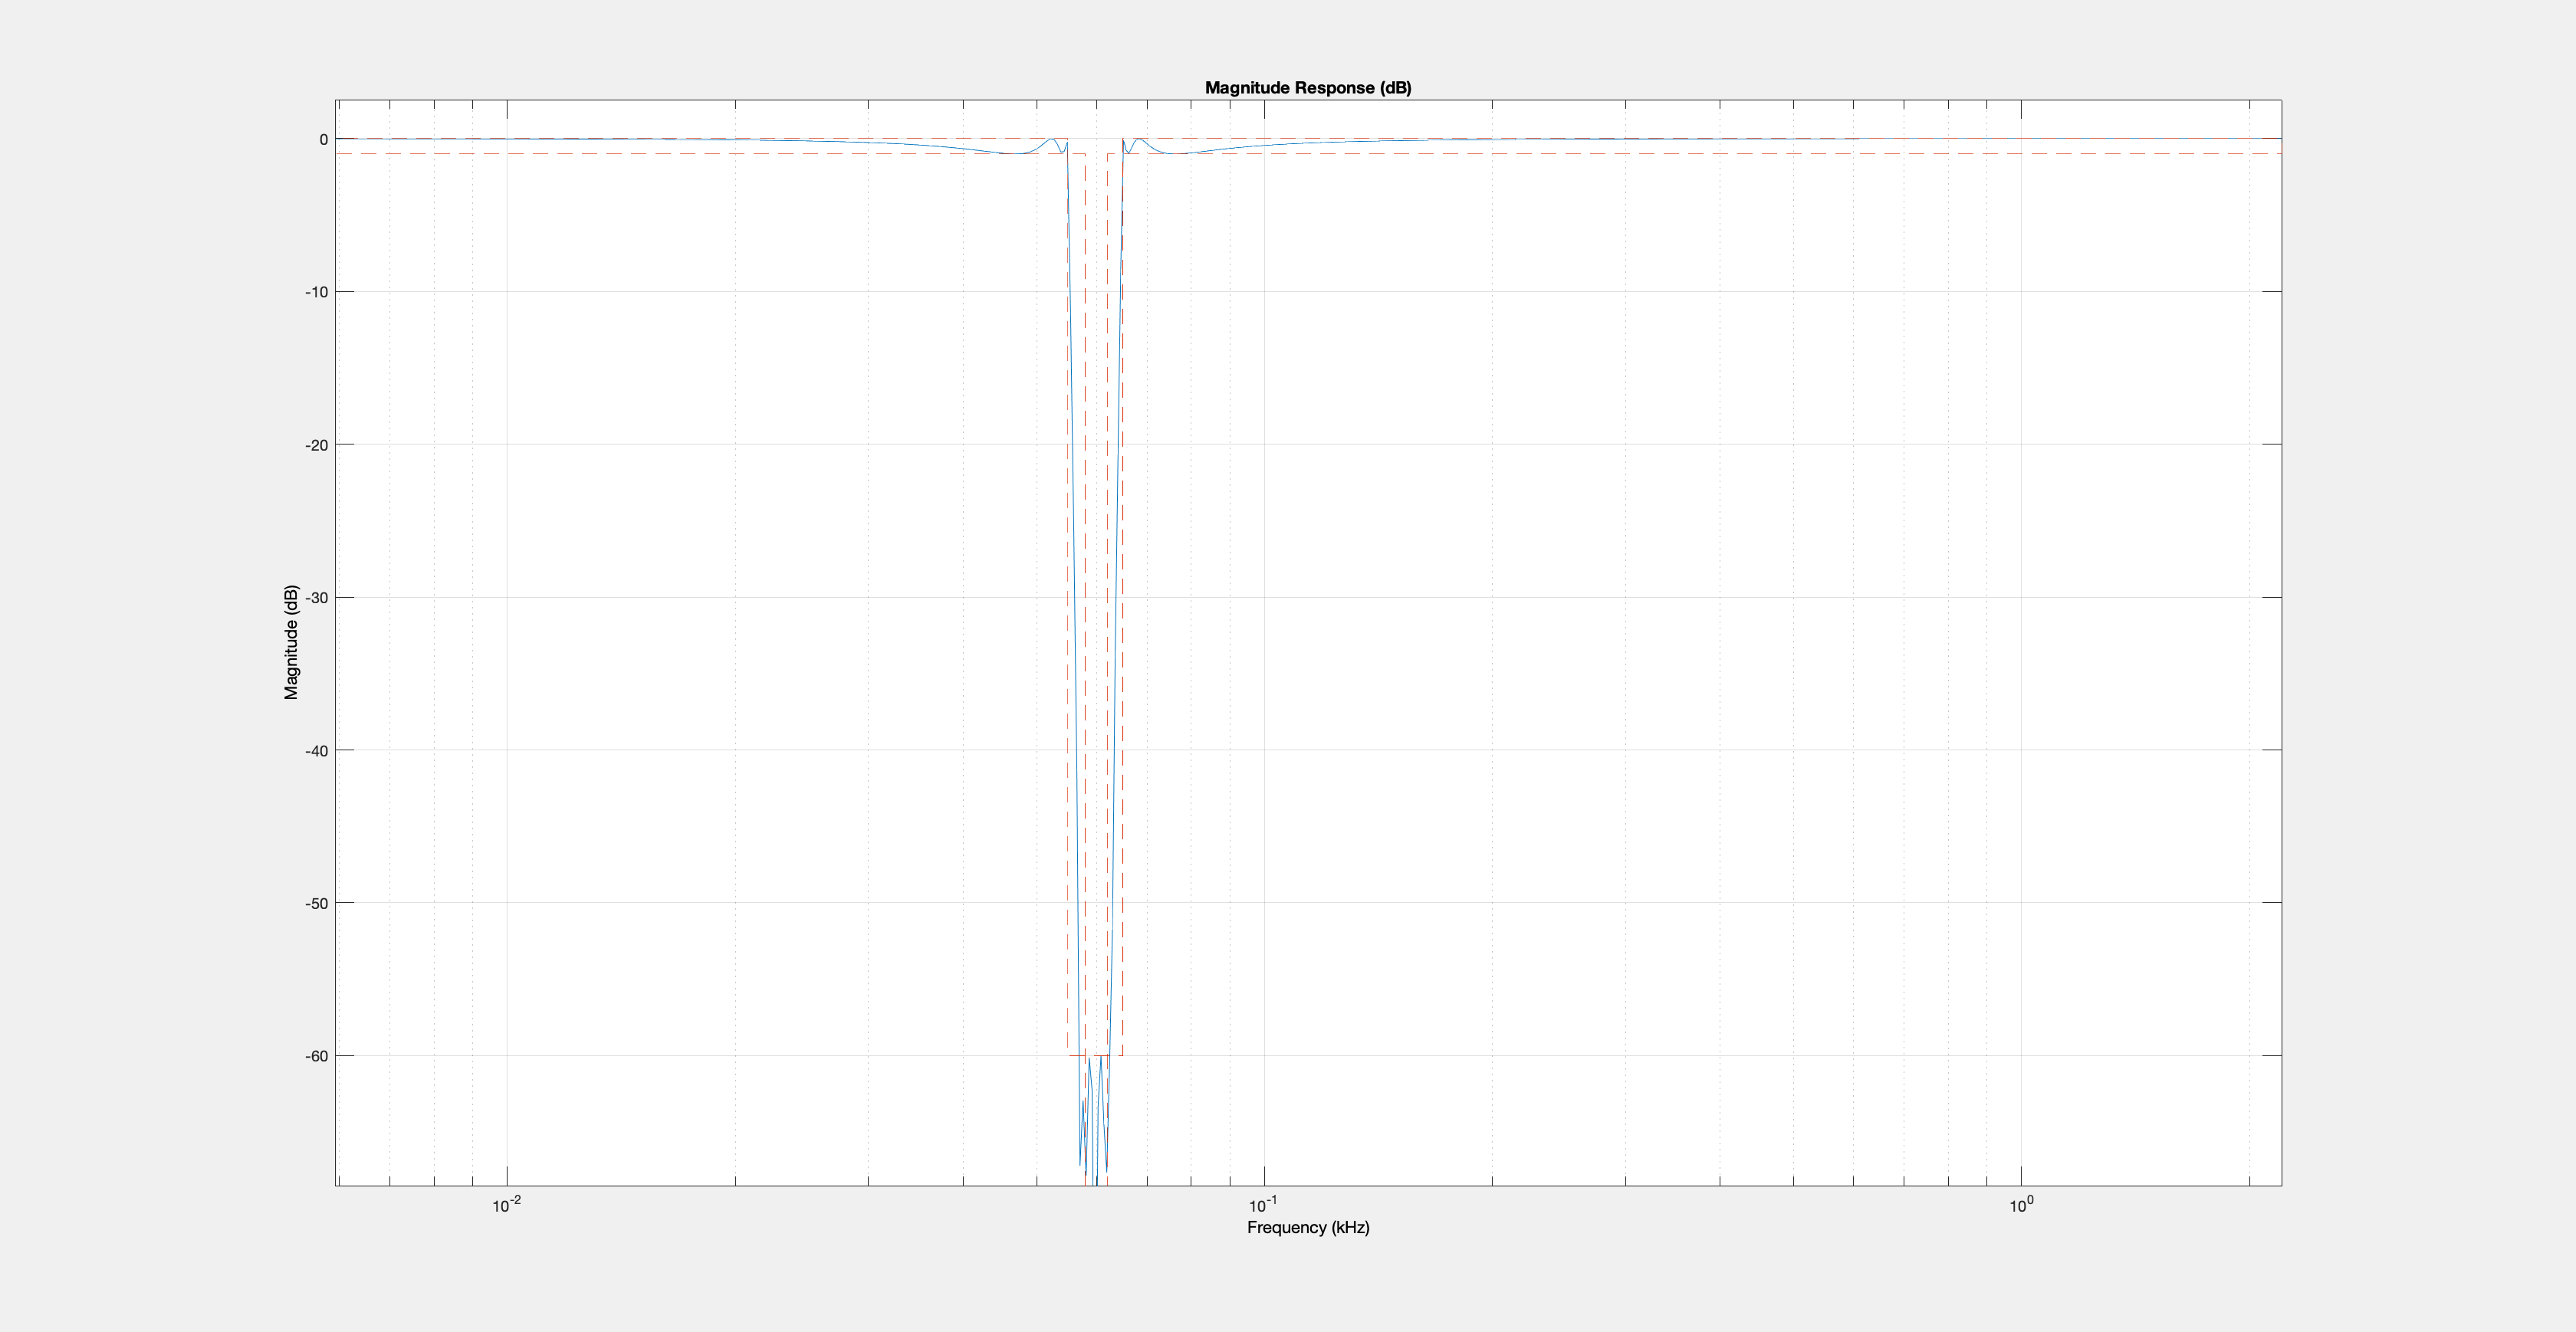
\includegraphics[width=\maxwidth{123.13095835423984em}]{figure_8}
\end{center}


\begin{par}
\begin{flushleft}
Perform zero-phase filtering to avoid distortion.
\end{flushleft}
\end{par}

\begin{matlabcode}
ybs = filtfilt(df,yds);
\end{matlabcode}


\begin{par}
\begin{flushleft}
Finally, upsample the signal to bring it back to the original audio sample rate of 44.1 kHz which is compatible with audio soundcards.
\end{flushleft}
\end{par}

\begin{matlabcode}
yf = interp(ybs,10);
Fs = Fs*10;
\end{matlabcode}


\begin{par}
\begin{flushleft}
Take a final look at the spectrum of the original and processed signals. Notice how the high frequency noise floor and the 60 Hz tone have been attenuated by the filters.
\end{flushleft}
\end{par}

\begin{matlabcode}
[Pfinal,Ffinal] = pwelch(yf,ones(8192,1),8192/2,8192,Fs,'power');
close(hfvt)
helperFilterIntroductionPlot1(F,P,Ffinal,Pfinal,...
  {'Original signal','Final filtered signal'})
\end{matlabcode}
\begin{center}
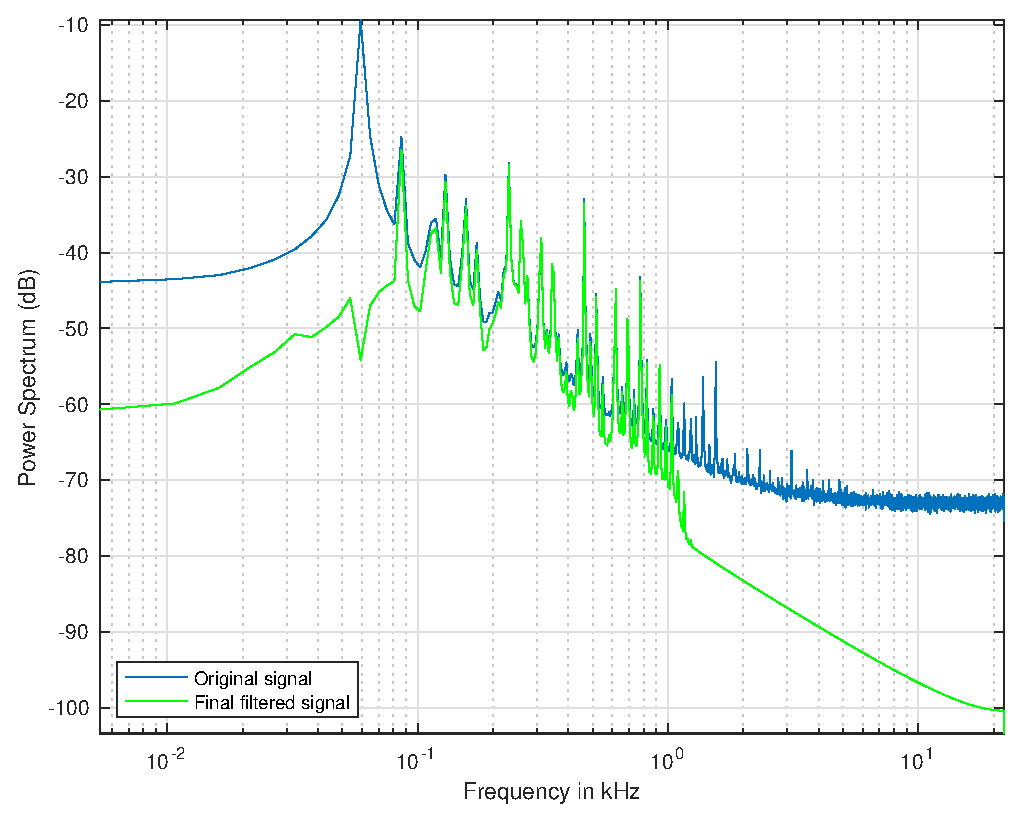
\includegraphics[width=\maxwidth{56.196688409433015em}]{figure_9}
\end{center}


\begin{par}
\begin{flushleft}
Listen to the signal before and after processing. As mentioned above, the end result is that you have effectively attenuated the 60 Hz hum and the high frequency noise on the audio file.
\end{flushleft}
\end{par}

\begin{matlabcode}
% Play the original signal 
hplayer = audioplayer(y, Fs);
play(hplayer);

% Play the noise-reduced signal
hplayer = audioplayer(yf, Fs);
play(hplayer);
\end{matlabcode}


\matlabheading{Differentiating a Signal}

\begin{par}
\begin{flushleft}
The MATLAB \textbf{diff} function differentiates a signal with the drawback that you can potentially increase the noise levels at the output. A better option is to use a differentiator filter that acts as a differentiator in the band of interest, and as an attenuator at all other frequencies, effectively removing high frequency noise.
\end{flushleft}
\end{par}

\begin{par}
\begin{flushleft}
As an example, analyze the speed of displacement of a building floor during an earthquake. Displacement or drift measurements were recorded on the first floor of a three story test structure under earthquake conditions and saved in the quakedrift.mat file. The length of the data vector is 10e3, the sample rate is 1 kHz, and the units of the measurements are cm. 
\end{flushleft}
\end{par}

\begin{par}
\begin{flushleft}
Differentiate the displacement data to obtain estimates of the speed and acceleration of the building floor during the earthquake. Compare the results using diff and an FIR differentiator filter.
\end{flushleft}
\end{par}

\begin{matlabcode}
load quakedrift.mat 

Fs  = 1000;                 % sample rate
dt = 1/Fs;                  % time differential
t = (0:length(drift)-1)*dt; % time vector
\end{matlabcode}


\begin{par}
\begin{flushleft}
Design a 50th order differentiator filter with a passband frequency of 100 Hz which is the bandwidth over which most of the signal energy is found. Set the stopband frequency of the filter to 120 Hz. 
\end{flushleft}
\end{par}

\begin{matlabcode}
df = designfilt('differentiatorfir','FilterOrder',50,...
                'PassbandFrequency',100,'StopbandFrequency',120,...
                'SampleRate',Fs);
\end{matlabcode}


\begin{par}
\begin{flushleft}
The \textbf{diff} function can be seen as a first order FIR filter with response $H(Z) = 1 - Z^{-1}$. Use FVTool to compare the magnitude response of the 50th order differentiator FIR filter and the response of the \textbf{diff} function. Clearly, both responses are equivalent in the passband region (from 0 to 100 Hz). However, in the stopband region, the 50th order filter attenuates components while the diff response amplifies components. This effectively increases the levels of high frequency noise.
\end{flushleft}
\end{par}

\begin{matlabcode}
hfvt = fvtool(df,[1 -1],1,'MagnitudeDisplay','zero-phase','Fs',Fs);
legend(hfvt,'50th order FIR differentiator','Response of diff function');
\end{matlabcode}
\begin{center}
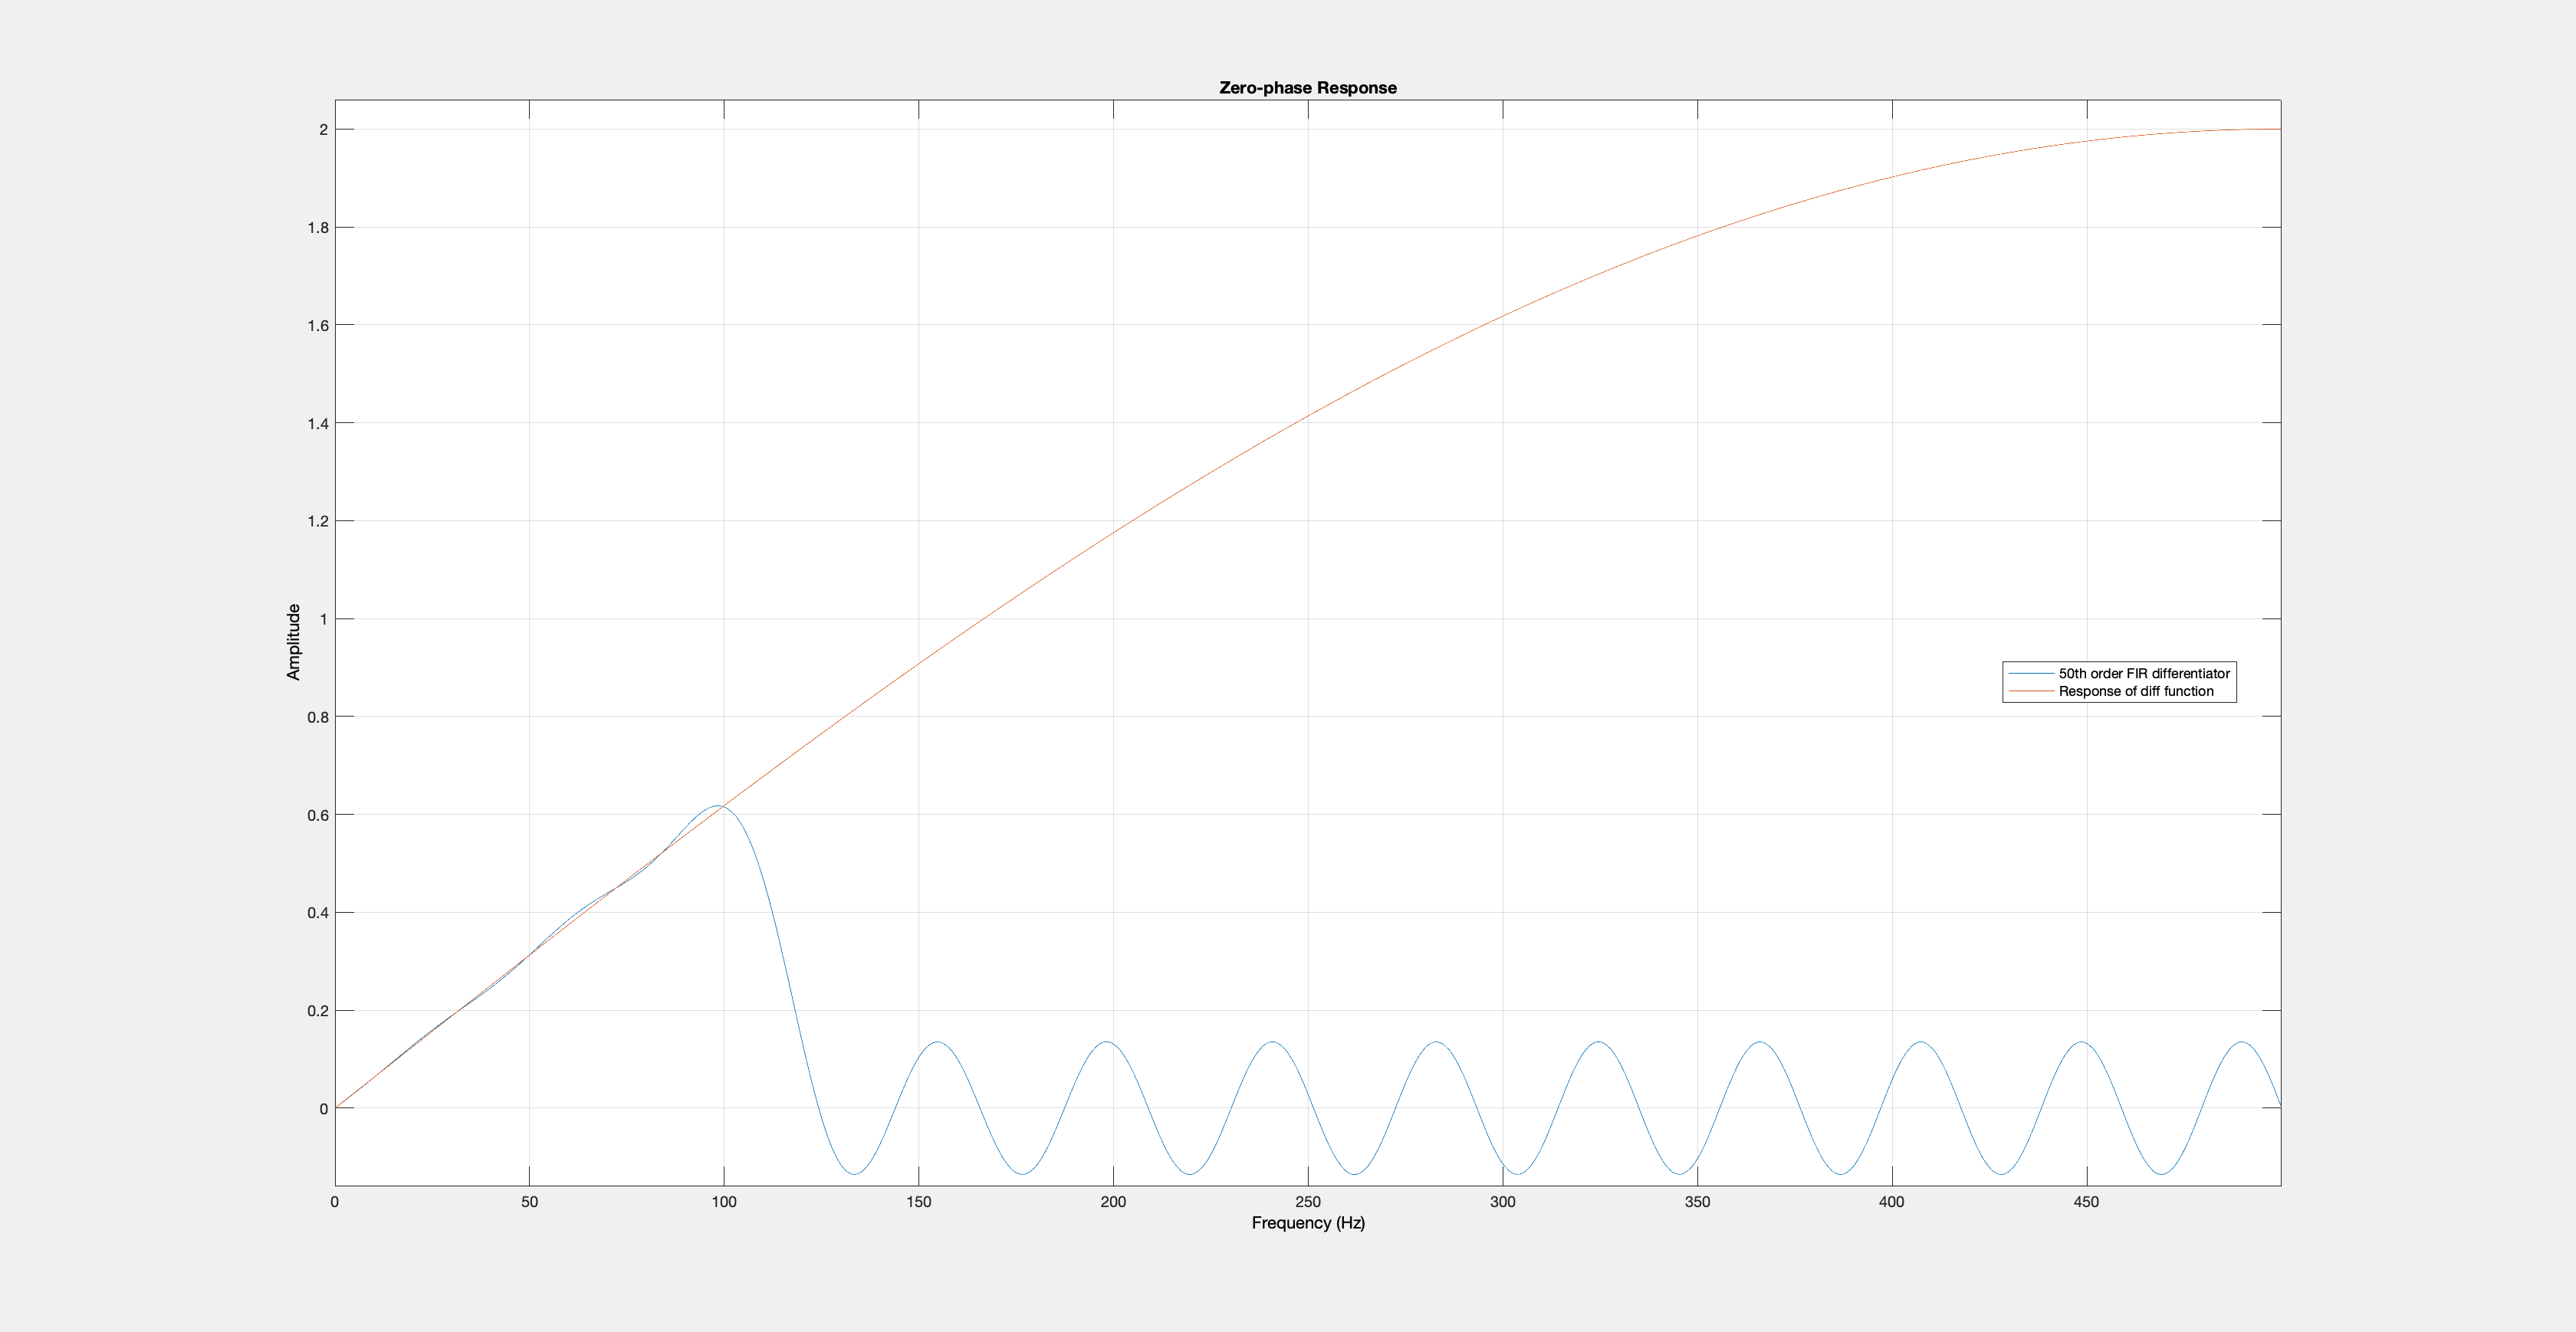
\includegraphics[width=\maxwidth{123.13095835423984em}]{figure_10}
\end{center}


\begin{par}
\begin{flushleft}
Differentiate using the \textbf{diff} function. Add zeros to compensate for the missing samples due to the diff operation.
\end{flushleft}
\end{par}

\begin{matlabcode}
v1 = diff(drift)/dt;
a1 = diff(v1)/dt;

v1 = [0; v1];
a1 = [0; 0; a1];
\end{matlabcode}


\begin{par}
\begin{flushleft}
Differentiate using the 50th order FIR filter and compensate for delay.
\end{flushleft}
\end{par}

\begin{matlabcode}
D = mean(grpdelay(df)); % filter delay
v2 = filter(df,[drift; zeros(D,1)]);
v2 = v2(D+1:end);
a2 = filter(df,[v2; zeros(D,1)]);
a2 = a2(D+1:end);
v2 = v2/dt;
a2 = a2/dt^2;
\end{matlabcode}


\begin{par}
\begin{flushleft}
Plot a few data points of the floor displacement. Plot also a few data points of the speed and acceleration as computed with diff and with the 50th order FIR filter. Notice how the noise has been slightly amplified in the speed estimates and largely amplified in the acceleration estimates obtained with \textbf{diff}.
\end{flushleft}
\end{par}

\begin{matlabcode}
helperFilterIntroductionPlot2(t,drift,v1,v2,a1,a2)
\end{matlabcode}
\begin{center}
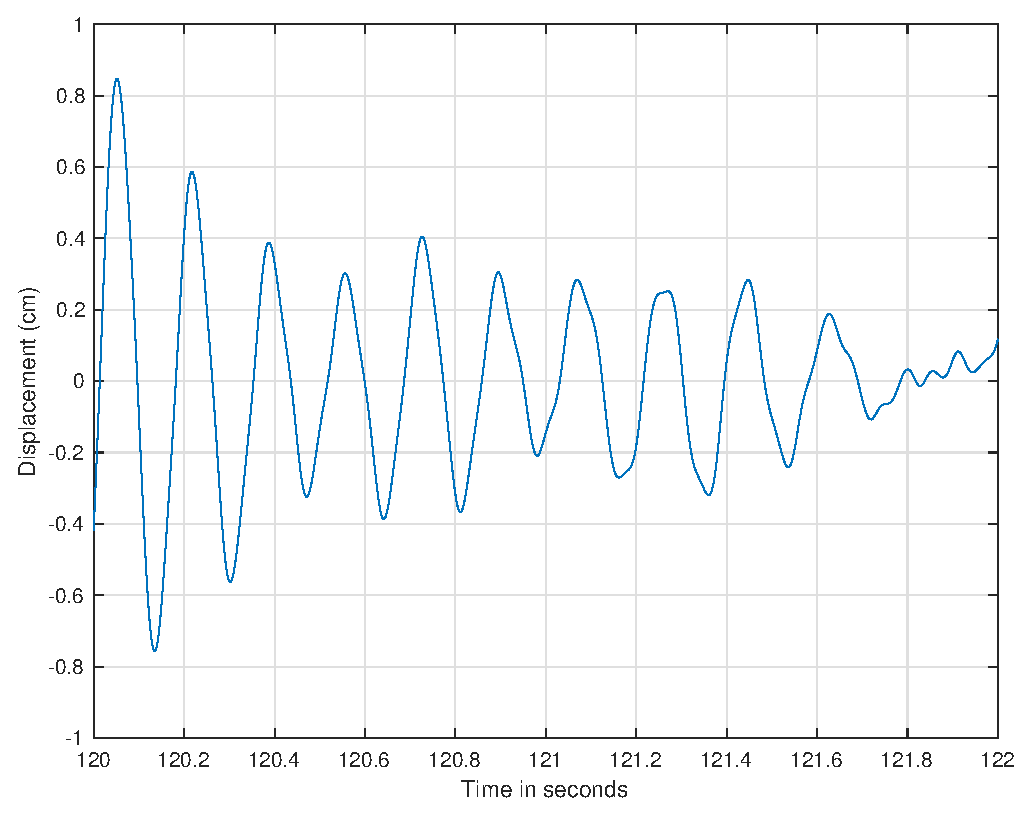
\includegraphics[width=\maxwidth{56.196688409433015em}]{figure_11}
\end{center}

\begin{center}
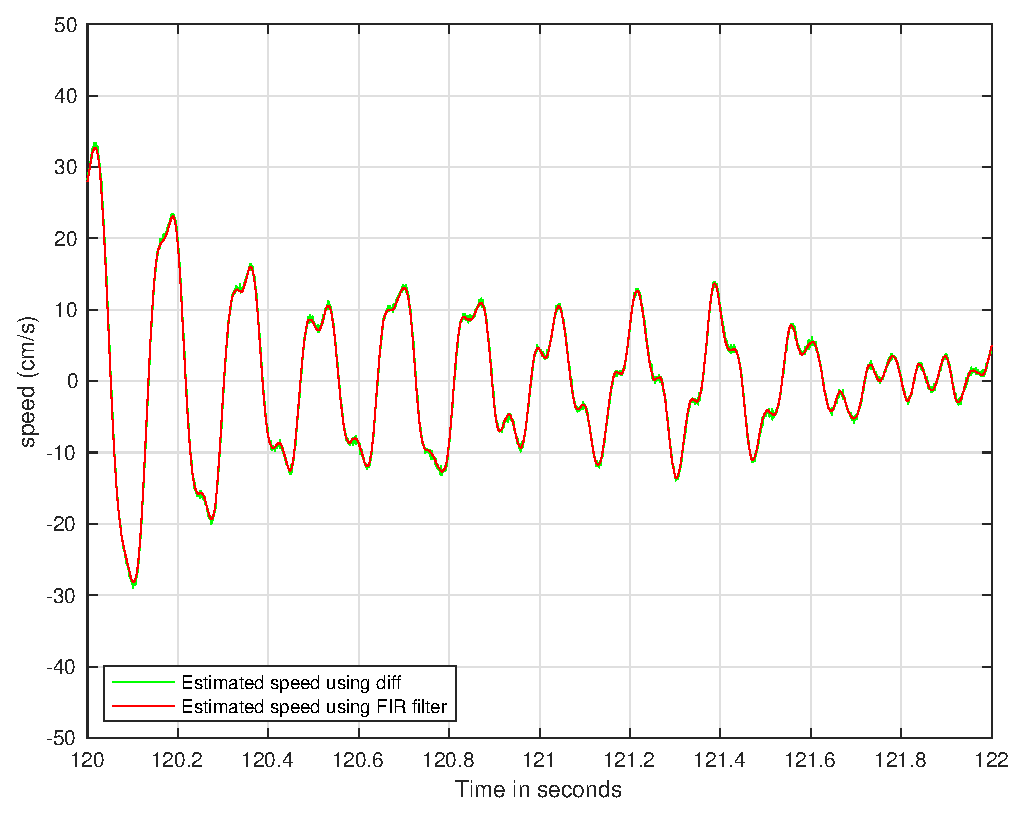
\includegraphics[width=\maxwidth{56.196688409433015em}]{figure_12}
\end{center}

\begin{center}
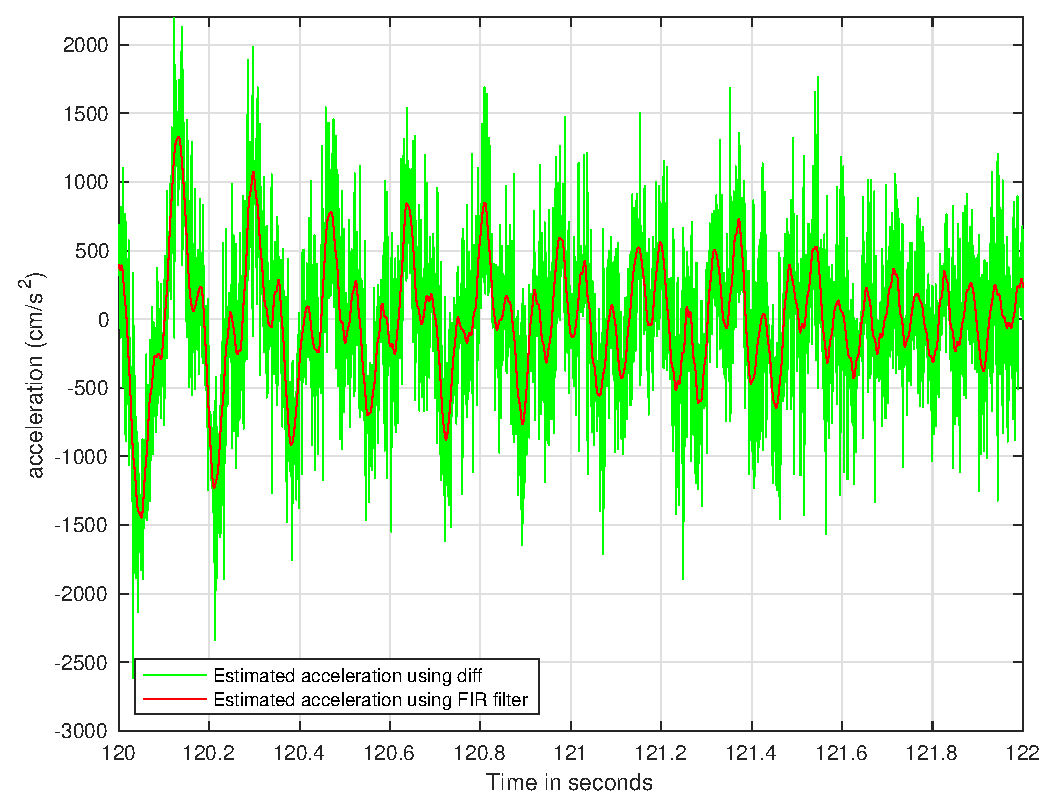
\includegraphics[width=\maxwidth{56.196688409433015em}]{figure_13}
\end{center}


\matlabheading{Integrating a Signal}

\begin{par}
\begin{flushleft}
A leaky integrator filter is an all-pole filter with transfer function $H(Z) = 1/[1-cZ^{-1}]$ where $c$ is a constant that must be smaller than 1 to ensure stability of the filter. It is no surprise that as $c$ approaches one, the leaky integrator approaches the inverse of the \textbf{diff} transfer function. Apply the leaky integrator to the acceleration and speed estimates obtained in the previous section to get back the speed and the drift respectively. Use the estimates obtained with the \textbf{diff} function since they are noisier.
\end{flushleft}
\end{par}

\begin{par}
\begin{flushleft}
Use a leaky integrator with $a = 0.999$. Plot the magnitude response of the leaky integrator filter. Notice that the filter acts as a lowpass filter effectively eliminating high frequency noise.
\end{flushleft}
\end{par}

\begin{matlabcode}
close(hfvt)
fvtool(1,[1 -.999],'Fs',Fs)
\end{matlabcode}
\begin{center}
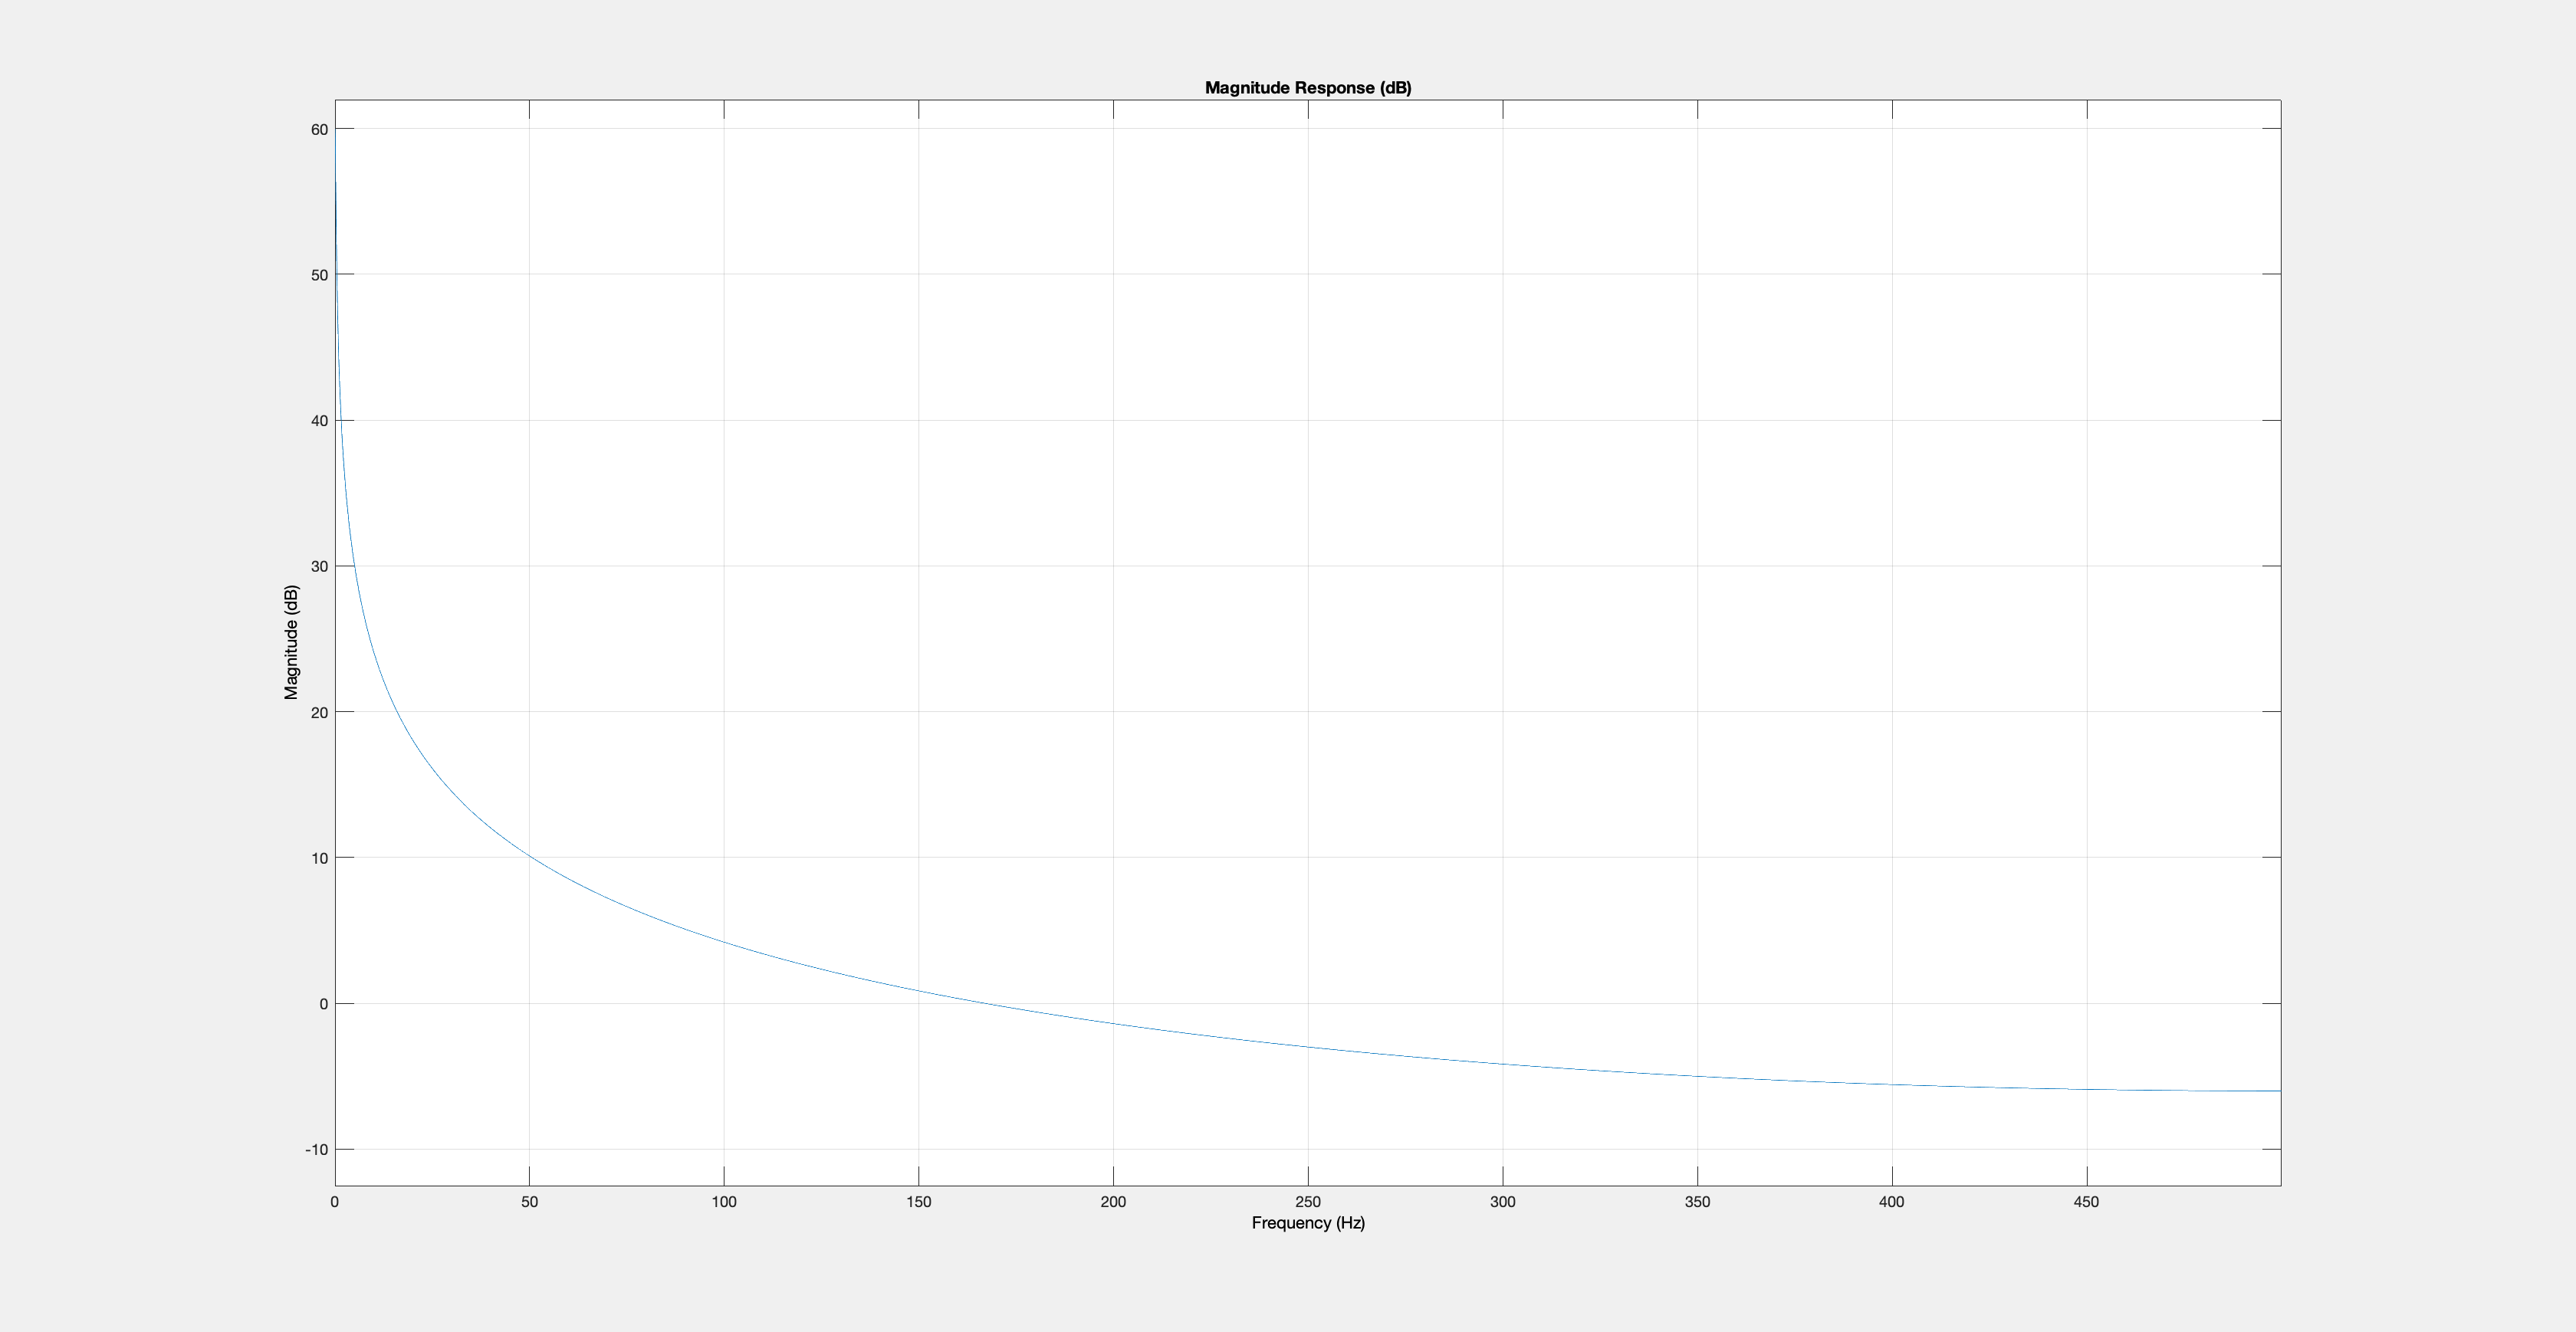
\includegraphics[width=\maxwidth{123.13095835423984em}]{figure_14}
\end{center}


\begin{par}
\begin{flushleft}
Filter the velocity and acceleration with the leaky integrator.
\end{flushleft}
\end{par}

\begin{matlabcode}
v_original = v1;
a_original = a1;

d_leakyint = filter(1,[1 -0.999],v_original);
v_leakyint = filter(1,[1 -0.999],a_original);

% Multiply by time differential
d_leakyint = d_leakyint * dt;
v_leakyint = v_leakyint * dt;
\end{matlabcode}


\begin{par}
\begin{flushleft}
Plot the displacement and speed estimates and compare to the original signals v1 and a1. 
\end{flushleft}
\end{par}

\begin{matlabcode}
helperFilterIntroductionPlot3(t,drift,d_leakyint,v_original,v_leakyint)
\end{matlabcode}
\begin{center}
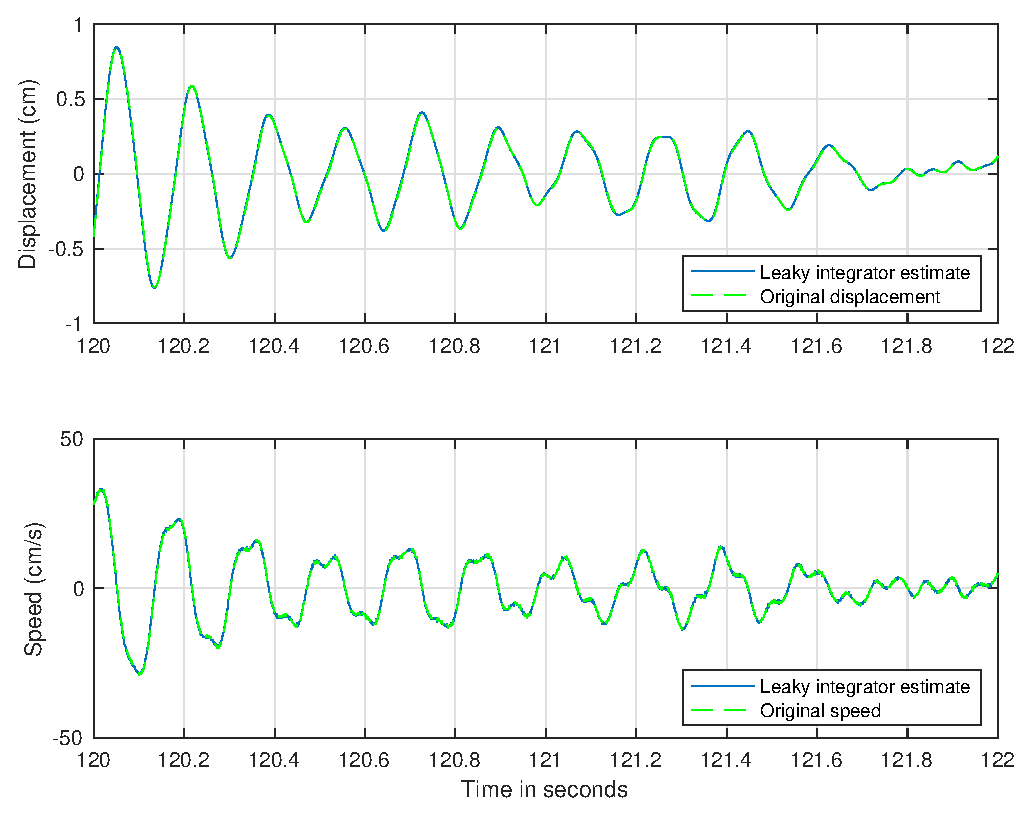
\includegraphics[width=\maxwidth{56.196688409433015em}]{figure_15}
\end{center}

\begin{par}
\begin{flushleft}
You can also integrate a signal using the \textbf{cumsum} and \textbf{cumtrapz} functions. Results will be similar to those obtained with the leaky integrator.
\end{flushleft}
\end{par}


\matlabheading{Conclusions}

\begin{par}
\begin{flushleft}
In this example you learned about linear and nonlinear phase filters and you learned how to compensate for the phase delay introduced by each filter type. You also learned how to apply filters to remove unwanted frequency components from a signal, and how to downsample a signal after limiting its bandwidth with a lowpass filter. Finally, you learned how to differentiate and integrate a signal using digital filter designs. Throughout the example you also learned how to use analysis tools to look at the response and group delay of your filters.
\end{flushleft}
\end{par}

\matlabheading{Further Reading}

\begin{par}
\begin{flushleft}
For more information on filter applications see the Signal Processing Toolbox. For more information on how to design digital filters see the \href{../../../signal/sigdemos/html/FilterDesignIntroductionExample.html}{"Practical Introduction to Digital Filter Design"} example.
\end{flushleft}
\end{par}

\begin{par}
\begin{flushleft}
References: J.G. Proakis and D. G. Manolakis, "Digital Signal Processing. Principles, Algorithms, and Applications", Prentice-Hall, 1996.
\end{flushleft}
\end{par}

\begin{par}
\begin{flushleft}
S. J. Orfanidis, "Introduction To Signal Processing", Prentice-Hall, 1996.
\end{flushleft}
\end{par}

\matlabheading{Appendix}

\begin{par}
\begin{flushleft}
The following helper functions are used in this example.
\end{flushleft}
\end{par}

\begin{itemize}
\setlength{\itemsep}{-1ex}
   \item{\begin{flushleft} \href{matlab:edit('helperFilterIntroductionPlot1.m')}{helperFilterIntroductionPlot1.m} \end{flushleft}}
   \item{\begin{flushleft} \href{matlab:edit('helperFilterIntroductionPlot2.m')}{helperFilterIntroductionPlot2.m} \end{flushleft}}
   \item{\begin{flushleft} \href{matlab:edit('helperFilterIntroductionPlot3.m')}{helperFilterIntroductionPlot3.m} \end{flushleft}}
\end{itemize}

\begin{par}
\begin{flushleft}
\textit{Copyright 2012-2013 The MathWorks, Inc.}
\end{flushleft}
\end{par}

\end{document}
